\cotefile{83}
\scanpage{178}
l'homomorphisme voulu de
\[
\deleted{\unsure{f}}\quad E_1\mathbin{*}_{\lambda}E_2\quad\text{dans}\quad E_1^\circ * E_2^\circ.
\]
Par passage à la limite \unsure{etc.}, on en conclut l'injectivité si les $F_i$ sont plats.

Il faut définir un $\lambda$-\unsure{semi-hom.} \inserted{(\uline{canonique}) sur} $\mathop{*}E_i$, donc il faut définir
\[
\mathop{*}^{i}E_i\longrightarrow\bigotimes E_i^\circ
\]
qui sur $\bigotimes E_i^\circ$ prenne la valeur $\lambda\,\mathrm{id}$.
Il faut donc trouver un $\lambda$-accouplement \unsure{canon. $i$-linéaire} dans $\bigotimes E_i^\circ$.

On songe \deleted{\unsure{tout}} de suite à :
\[
f=\bigotimes u_i:\ \bigotimes E_i\longrightarrow\bigotimes E_i^\circ
\]
\[
f(x_1,\ldots x_n)=u_1(x_1)\otimes\cdots\otimes u_n(x_n)
\]
\[
\begin{aligned}
f(x_1+\alpha_1,x_2\ldots x_n)
 &=\bigl(u_1(x_1)+\lambda\alpha_1\bigr)\otimes u_2(x_2)\cdots\otimes u_n(x_n)\\
 &=f(x_1,\ldots x_n)+\underbrace{\lambda\alpha_1}_{\deleted{\unsure{\alpha_1}}}\otimes u_2(x_2)\cdots u_n(x_n)
\end{aligned}
\]
\margin{mais il faudrait remplacer $\bigotimes E_i$ par son \unsure{im.} --- ou bien ne pas \unsure{considérer} dans les données
\diagram{\begin{tikzcd}[ampersand replacement=\&]F_i\arrow[r,"\unsure{v_i}"]\&E_i\end{tikzcd}}
\unsure{pour celles qui sont} injectives mais seulement \unsure{se donner un} $u_i:E_i\unsure{\to|-}F_i$ \unsure{avec} $u_i\unsure{v_i}=\lambda\,\mathrm{id}_{F_i}$.}

prendre donc comme application associée
\[
f^\circ(\alpha_1,\ldots,\alpha_n)=\lambda\alpha_1\otimes\cdots\otimes\alpha_n
\]
de sorte que les termes \unsure{en nb premiers} \inserted{\unsure{d'ordre}}\margin{177}
\scanpage{179}
Ceci dit, pour définir \inserted{un} $f$ \deleted{$\unsure{f^\circ}$} correspondant à un $f^\circ$ déjà donné, on peut se le donner arbitrairement \inserted{\unsure{(soit $g$)}} sur $\prod F_i$ (comme applic\unsure{ation} multilin.).

\deleted{On \unsure{aura donc}}
Faisons le calcul pour deux facteurs ---
On pose (avec $x_i\in F_i$, $\alpha_i\in E_i^\circ$)
\[
\begin{aligned}
f(\underbrace{x_1+\alpha_1}_{X_1},\underbrace{x_2+\alpha_2}_{X_2})
 &=g(x_1,x_2)+\deleted{\unsure{f(x_1,\alpha_2)}}f^\circ(\alpha_1,b_2(x_2))\\
 &\quad+f^\circ(b_1(x_1),\alpha_2)
 +\underbrace{\lambda f^\circ(\alpha_1,\alpha_2)}_{\substack{\Vert\\f^\circ(u_1(\alpha_1),\alpha_2)\\=f^\circ(\alpha_1,u_2(\alpha_2))}}
\end{aligned}
\]
Il suffit de vérifier que ça satisfait aux deux conditions. P. ex si on remplace $\alpha_1$ \deleted{\unsure{par}} $\alpha_1+\alpha'_1$, on obtient
\[
\begin{aligned}
f(X_1+\alpha'_1,X_2)&=f(X_1,X_2)+f^\circ(\alpha'_1,\uline{b_2(x_2)})\\
&\qquad+\lambda f^\circ(\alpha'_1,\alpha_2)
\end{aligned}
\]
et on \unsure{veut}
\[
=f(\unsure{x_1|X_1},X_2)+f^\circ\bigl(\alpha'_1,\underbrace{u_2(X_2)}_{b_2(x_2)+\lambda\alpha_2}\bigr)\qquad\text{OK.}
\]
Prenant pour $B$ le produit tensoriel $E_1^\circ\otimes E_2^\circ$, pour $f^\circ$ l'accouplement can., et $g=0$, on trouve
\margin{178}
\scanpage{180}
\[
f^\circ(\alpha_1,u_2(x_2),\ldots,u_n(x_n)).
\]
\margin{\uline{NB} Si les \deleted{\unsure{ext.}} $E_i$ sont munis de scindages et leurs structures de $\lambda$-triv. définies par des $\unsure{b_i}:F_i\unsure{\to|-}E_i^\circ$, alors la $\lambda$-trivialisation de $\mathop{*}E_i$, scindé de la façon \unsure{can.}, est donnée par $\bigotimes b_i:\bigotimes F_i\unsure{\to|-}\bigotimes E_i^\circ$.}
Ainsi, on a une opération interne $*$ dans la catégorie des extensions $\lambda$-scindées \inserted{(à quotients $F_i$ plats, au besoin)}, et en particulier dans celle des torseurs $\lambda$-scindés (car si les $F_i$ sont $\simeq k$, $\bigotimes F_i\simeq k$ canon.\unsure{t}).

\deleted{\unsure{O}}\unsure{outre} les \unsure{données} de commutativité, d'associativité (à vérifier leurs compatibilités !), a-t-on une unité ?

Il faudrait pour le moins, \deleted{que} pour une unité,
\diagram{\begin{tikzcd}[ampersand replacement=\&]0\arrow[r,dash]\&E^\circ\arrow[r,dash]\&E\arrow[r,dash]\&F\arrow[r]\&0\end{tikzcd}}
que $E^\circ$, et $F$ soient unités pour le $\otimes$ ordinaire, donc \deleted{inversibles} \inserted{$\simeq k$}.
\diagram{\begin{tikzcd}[ampersand replacement=\&]0\arrow[r]\&k\arrow[r]\&E\arrow[r]\&k\arrow[r]\&0\end{tikzcd}}
\deleted{\unsure{Donc les}} \unsure{Choisissons} scindage, alors la $\lambda$-triv. est définie par
\[
\deleted{\unsure{k\to k}}:\ k\longrightarrow k\qquad\text{i.e. }\beta_0\in k
\]
J'ai envie de prendre $\beta_0=1$. Prenons plus généralement $\beta$ quelconque, je dis qu'alors
\[
E_\beta\mathbin{*}_{\lambda}E_2\simeq {}^\beta E_2,
\]
muni de la $\lambda$ \inserted{trivialisation $\beta u_2$ déduite de celle de $E_2$}
\margin{179}
\scanpage{181}
Ce foncteur $E\unsure{\to|-}{}^\beta E$ \deleted{\unsure{e}} est une équivalence de cat ssi $\beta$ est inversible dans $k$ --- Et si $\beta=1$, on retrouve ${}^1E=E$.

En termes intrinsèques, pour \deleted{que} un $M$ $\lambda$-trivialisé, les conditions suivantes sont équivalentes

1) $M\mathbin{*}_{\lambda}\,?$ est une équivalence sur la cat. des $\lambda$-trivialisations

2) $M^\circ\unsure{\to|-}M$ injectif, $\underset{L''}{M^\circ}$ et $\underset{L'}{M/M^\circ}$ inversibles,
\[
M\xrightarrow{u}M^\circ\quad\text{est surjectif}
\]
(en termes de \deleted{$\unsure{M/M^\circ}$} un scindage cela signifie que l'idéal somme \inserted{des images de}
\[
L'\otimes\unsure{L''}^{-1}\xrightarrow{\beta}k
\]
et $\lambda k$ est $k$)

3) $M$ inv. pour $\mathbin{*}_{\lambda}$
\margin{180}
\scanpage{183}
\mspage{I bis}
\margin{Mai 1986\\Juillet 1986}
$\unsure{\mathcal{A}|A}$ alg. d'Az. de rang $4$ sur $k$, on veut expliciter sa structure multiplicative en termes de la forme $\det$, de l'élément $1$, et de la structure \uline{spéciale} orthogonale $e\in\bigwedge^4\mathcal{A}$ can. \deleted{\unsure{associée}} associée à $\det$ ($e\otimes e=\operatorname{dis}(\det)$).
Comme on connaît la forme $\operatorname{Tr}xy$ par la formule
\margin{\uline{NB} $\operatorname{Tr}$ connu en termes de $\det$ et de $1$, comme $\operatorname{Tr}(x)=\Psi_{\det}(x,1)$ i.e.}
\[
\det(x+y)=\det x+\det y+\operatorname{Tr}x\operatorname{Tr}y-\operatorname{Tr}xy
\]
\[
\Psi_{\det\deleted{\unsure{(xy)}}}(x,y)=\operatorname{Tr}x\operatorname{Tr}y-\underbrace{\operatorname{Tr}xy}_{\varphi(x,y)},
\]
\deleted{pour} et que celle-ci est non dég., pour connaître $xy$, il suffit de connaître
\[
\operatorname{Tr}xyz\qquad\forall z\in\mathcal{A}.
\]
Donc je cherche une formule pour $\operatorname{Tr}xyz$. Comme $\operatorname{Tr}(xy)z$ et $\operatorname{Tr}(yx)z$ ne sont pas égaux en général, i.e la structure mult\inserted{de $\mathcal{A}$} n'est pas commutative \deleted{(donc} On voit que $\det,1$ sans $e$ ne suffisent à expliciter $\operatorname{Tr}xyz$ (car ils ne déterminent la structure multiplicative que mod passage à l'inverse, i.e. mod l'involution
\[
x\longmapsto x'=\operatorname{Tr}(x).1-x.
\]
On note aussi que $\operatorname{Tr}xyz$ ne dépend que du triple $\{x,y,z\}$ et d'un ordre circulaire sur l'\unsure{ens.} des trois termes. On a, \deleted{pour} si
\[
\begin{aligned}
\tau&=\operatorname{Tr}xyz\quad(=\operatorname{Tr}yzx=\operatorname{Tr}zxy)\\
\tau'&=\operatorname{Tr}(zyx)\bigl(=\operatorname{Tr}(yxz)=\operatorname{Tr}(xzy)\bigr)
\end{aligned}
\]
\margin{182}
\scanpage{184}
\margin{\(\begin{array}{lll}\operatorname{Tr}x=b&\operatorname{Tr}y=b'&\operatorname{Tr}z=b''\\\det x=c&\det y=c'&\det z=c''\\\operatorname{Tr}yz=t&\operatorname{Tr}zx=t'&\operatorname{Tr}xy=t''\end{array}\)}
la formule
\[
\tau+\tau'=\operatorname{Tr}(xy+yx)z\qquad\text{où}
\]
\[
xy+yx=\underbrace{\operatorname{Tr}(y)}_{b'}x+\underbrace{\operatorname{Tr}(x)}_b y+\bigl(\underbrace{\operatorname{Tr}(xy)}_{t''}.\unsure{1}-\underbrace{\operatorname{Tr}x}_b\underbrace{\operatorname{Tr}y}_{b'}\bigr)1
\]
donc
\[
\deleted{\unsure{(xy)z+}}\quad
(xy+yx)z=b'xz+byz+(t''-bb')z\qquad\text{d'où}
\]
\[
\boxed{\tau+\tau'=\unsure{bt|b''t''}+b't'+b''t''-bb'b''}
\overset{\mathrm{def}}{=}\Sigma(b,b',b'',t,t',t'')
\]
On devine que $\tau\tau'$ sera également un polynôme en $b,b',b'',c,c',c'',t,t',t''$, de sorte que $\tau,\tau'$ s'expliciteront (à permutation près) comme racines d'un polynôme \inserted{unitaire} du second degré, dont les coeff $B$ ($=\tau+\tau'$) et $C$ ($=\tau\tau'$) sont des polynômes en les variables $\uline{b^{(i)}},\uline{c^{(i)}},\uline{t^{(i)}}$.

\deleted{Mais plutôt que de chercher une expression pour $\tau\tau'$, je vais essayer de les \inserted{($\tau$ et $\tau'$)} déterminer directement en termes de $\det,1$ \uline{et de $e$}.
Je suis guidé par le fait que $xy$ et $yx$ sont opposés mod $1,x,y$ --- donc \uline{si $z$ est orth.} à $1,x,y$ \deleted{\unsure{det}} \inserted{(pour $\varphi$)} on aura
\[
\operatorname{Tr}(xyz)=-\operatorname{Tr}(yxz).
\]
Pour se ramener à ce cas, on construit $\alpha,\beta,\gamma\in k$ tels que
\[
z'=z-\alpha1-\beta x-\gamma y
\]
soit orth. à $1,x,y$, i.e.
\[
\begin{aligned}
b''-2\alpha-b\beta-b'\gamma&=0\\
t'-\unsure{b}\alpha+(2c-b^2)\beta-t''\gamma&=0\\
t-\deleted{\unsure{b\alpha}}\inserted{b'\alpha}-t''\beta+(2c'-b'^2)\gamma&=0
\end{aligned}
\]
i.e
\[
\left\{\begin{aligned}
2\alpha+b\beta+b'\gamma&=b''\\
b\alpha+(b^2-2c)\beta+t''\gamma&=t'\\
b'\alpha+t''\beta+(b'^2-2c')\gamma&=t
\end{aligned}\right.
\]
matrice
\diagram{\(\begin{pmatrix}2&b&b'\\b&b^2-2c&t''\\b'&t''&b'^2-2c'\end{pmatrix}\)}
}
\margin{183}
\scanpage{185}
avec donc
\[
(1\wedge x\wedge y\wedge z)\otimes e^{-1}=2\varepsilon_0
\]
\margin{$\varepsilon_0=\bigl[\alpha\wedge\alpha'\wedge x_0\wedge y_0\bigr)\unsure{e^{-1}}\in\pm1$}
le signe dépend de la convention d'orient. (qu'il faudra préciser le moment venu !).

D'autre part
\[
\deleted{\operatorname{Tr}xyz=1}\qquad
\tau-\tau'=\operatorname{Tr}\underbrace{[x,y]}_z.z=\operatorname{Tr}z^2=\operatorname{Tr}1=2
\]
d'où
\[
2=2\varepsilon\varepsilon_0\qquad\text{i.e.}
\]
\[
\varepsilon=\deleted{\unsure{1}}\inserted{\unsure{\tfrac12}}\varepsilon_0\quad\deleted{\unsure{\varepsilon}}
\]
d'où
\[
\boxed{\tau-\tau'=\deleted{\unsure{1}}\inserted{\unsure{\tfrac12}}\varepsilon_0\underbrace{(1\wedge x\wedge y\wedge z)\otimes e^{-1}}_{\Delta\ \mathrm{def}}}
\quad\text{i.e. }2(\tau-\tau')=\varepsilon_0\Delta
\]
(a un sens si $2$ inv. dans l'anneau de base $k$ où on travaille).

On en tire
\[
4\tau\tau'=(\tau+\tau')^2-(\tau-\tau')^2=\Sigma^2-\deleted{\unsure{1}}\inserted{\unsure{\tfrac14}}\Delta^2
\]
À vérifier (dans $\mathbb{Q}[[\deleted{b,b',b''}\ x_{ij},y_{ij},z_{ij}]]$ $1\leq i,j\leq2$)
\[
\Sigma^2-\deleted{\unsure{1}}\inserted{\unsure{\tfrac14}}\Delta^2\in4\mathbb{Z}[b,b',b'',t,t',t'']
\]
\margin{?}
\deleted{i.e.}
\deleted{\[
4\Sigma^2-\Delta^2\in16\mathbb{Z}[b,b',b'',t,t',t'']
\]}
d'où l'expression
\[
\tau\tau'=\Pi(b,b',b'',t,t',t'')\in\mathbb{Z}[b,b',b'',t,t',t'']
\]
expression polynomiale de poids total $6$ (les $b$ étant de
\margin{184}
\scanpage{186}
On va plutôt essayer de calculer
\[
\tau'-\tau=\operatorname{Tr}xyz-\operatorname{Tr}yxz
=\operatorname{Tr}([x,y]z)=\operatorname{Tr}([y,z]x)=\operatorname{Tr}([z,x].y)
\]
c'est une expression \inserted{multilin.} alternée en $x,y,z$, donc on doit avoir
\[
\tau'-\tau=\deleted{\unsure{\varepsilon}}(a\wedge x\wedge y\wedge z)\otimes e^{-1}
\]
pour $a\in\mathcal{A}$ bien déterminé. Comme cette expression est invariante par $G=\uline{\operatorname{Aut}}\mathcal{A}$, \deleted{on voit que} et que (si $g\in G(-)$)
\[
g(a)\wedge g(x)\wedge g(y)\wedge g(z)=a\wedge x\wedge y\wedge z\quad(=a\wedge g(x)\wedge g(y)\wedge g(z))
\]
on en conclut que $a=ga$ i.e. inv. sous $G$ i.e. $a=\varepsilon.1$. Donc on doit avoir
\[
\tau'-\tau=\varepsilon(1\wedge x\wedge y\wedge z)\otimes e^{-1}
\]
et pour calculer $\varepsilon$, il suffit de prendre $x,y,z$ tels que $1\wedge x\wedge y\wedge z$ inv. i.e. $1,x,y,z$ une base \inserted{de $\mathcal{A}$}. On prendra
\[
x_0=\begin{pmatrix}0&0\\1&0\end{pmatrix},\quad
y_0=\begin{pmatrix}0&1\\0&0\end{pmatrix},\quad
z_0=[x_0,y_0]=\begin{pmatrix}-1&0\\0&1\end{pmatrix}=1-2\alpha
\]
où $\alpha=\begin{pmatrix}1&0\\0&0\end{pmatrix}$
\[
\left(\mathrm{NB}\quad x_0y_0=\begin{pmatrix}0&0\\0&1\end{pmatrix},\quad y_0x_0=\begin{pmatrix}1&0\\0&0\end{pmatrix}\right)
\quad\deleted{\left(x_0y_0z_0=\begin{pmatrix}0&0\\0&1\end{pmatrix}\right)}
\]
On trouve
\[
1\wedge x_0\wedge y_0\wedge z_0=-2\,1\wedge x_0\wedge y_0\wedge\alpha
=-2\alpha'\wedge x_0\wedge y_0\wedge\alpha
=2\deleted{\unsure{x_0\wedge y_0\wedge\alpha\wedge\alpha'}}\inserted{\alpha\wedge\alpha'\wedge x_0\wedge y_0}
\]
où
\[
\alpha=\begin{pmatrix}1&0\\0&0\end{pmatrix},\quad\alpha'=\begin{pmatrix}0&0\\0&1\end{pmatrix}
\]
et \deleted{\unsure{x,y}} $\alpha,\alpha',x_0,y_0$ forment base can. de $M_2(\mathbb{Z})$. On
\margin{185}
\scanpage{187}
poids $1$ et les $t$ de poids $2$), et de poids total $2$ en chacune des \deleted{paires de} variables \inserted{$x,y,z$ ($x$ intervenant avec poids $1$ dans $b,t',t''$, poids $0$ dans $b',b'',t$)} \deleted{$(b,t),(b',t'),(b'',t'')$}.
De plus, il doit être symétrique par permutation des \deleted{\unsure{quatre}} \inserted{trois} paires de variables $(b,t),(b',t'),(b'',t'')$. Et idem pour $\Delta^2$.

On doit donc avoir
\[
\begin{aligned}
\Delta^2={}&\alpha tt't''+\deleted{\beta\bigl(b^2t't''+tb'^2t''+tt'b''^2\bigr)+\gamma\bigl(tb'^2b''^2+b^2t'b''^2+b^2b'^2t''\bigr)+\delta b^2b'^2b''^2}\\
&\deleted{\unsure{\gamma}\bigl(b'b''b^2\unsure{t}+b''bb'^2\unsure{t'}\bigr)}\\
&\inserted{\beta(b^2t^2+b'^2t'^2+b''^2t''^2)+\gamma(b'b''t't''+b''bt''t+bb'tt')}\\
&\inserted{{}+\delta(b'b''b^2t+b''bb'^2t'+bb'b''^2t'')+\unsure{\eta}b^2b'^2b''^2}
\end{aligned}
\]
avec
\[
\alpha,\beta,\gamma,\delta\in\mathbb{Z}
\]
à déterminer, par (quatre ?) choix particuliers judicieux des triples $(x,y,z)$. P. ex. le triple précédent $x_0,y_0,z_0=[x_0,y_0]$ donne $b,b',b''=0$, et $\Delta=2\varepsilon_0$, $\uline{\Delta^2=4}$, d'où
\[
4=\alpha tt't''
\]
où
\[
t''=\operatorname{Tr}x_0y_0=1,\quad t^{\deleted{\unsure{\circ}}}=\operatorname{Tr}y_0z_0=0,\quad t'=\operatorname{Tr}z_0x_0=0
\]
et on trouve $4=0.\alpha=0$, ce qui est fâcheux !

Et pour cause --- il faudra, dans l'expression de $\Delta^2$, faire intervenir aussi $c,c',c''$. En fait, on trouve immédiatement, une fois qu'on y pense :
\margin{186}
\scanpage{188}
\[
\Delta(x,y,z)^2=\det\begin{pmatrix}
\varphi(1,1)&\varphi(1,x)&\varphi(1,y)&\varphi(1,z)\\
\varphi(x,1)&\varphi(x,x)&\varphi(x,y)&\varphi(x,z)\\
\varphi(y,1)&\varphi(y,x)&\varphi(y,y)&\varphi(y,z)\\
\varphi(z,1)&\varphi(z,x)&\varphi(z,y)&\varphi(z,z)
\end{pmatrix}
\]
où $\varphi(u,v)$ est la forme bil. sym. associée à la forme quadratique $q$ ($=\det$)
\[
\varphi(u,v)=\operatorname{Tr}u\operatorname{Tr}v-\operatorname{Tr}(uv)=
\]
\uline{NB} On a
\[
\varphi(u,1)=\operatorname{Tr}(u)\quad\deleted{\unsure{\varphi(u,1)}}
\]
\[
\varphi(u,u)=2\det u
\]
Donc on trouve
\[
\boxed{\Delta(x,y,z)^2=\det\begin{pmatrix}
2&b&b'&b''\\
b&2c&bb'-t''&bb''-t'\\
b'&bb'-t''&2c'&b'b''-t\\
b''&bb''-t'&b'b''-t&2c''
\end{pmatrix}}
\]
ce qui permet d'expliciter
\[
4\tau\tau'=\Sigma^2-\Delta^2
\]
\margin{\unsure{où}}
où $\Delta$ est donné ci-dessus, et
\[
\boxed{\Sigma=bt+b't'+b''t''-bb'b''}
\]
\margin{187}
\scanpage{189}
Le calcul ``\unsure{bébête}'', en développant le déterminant et tenant compte des symétries (pour regrouper les termes qui se correspondent par \deleted{symétrie} op. de $\mathfrak{S}_3$) et $\Sigma^2$,
\[
\Sigma^2-\Delta^2=4\Pi(b,b',b'',t,t',t'',c,c',c'')
\]
avec
\[
\boxed{\begin{aligned}
\Pi={}&tt't''+(ct^2+c't'^2+c''t''^2)+(b^2c'c''+b'^2c''c+b''^2cc')\\
&-(b'b''ct+b''bc't'+bb'c''t'')
\end{aligned}}
\]
\inserted{\[
=tt't''+ct(t-b'b'')+c't'(t'-b''b)+c''t''(t''-bb')+(b^2c'c''+b'^2c''c+b''^2cc')
\]}
On aura donc
\[
\left\{\begin{aligned}
\tau+\tau'&=\Sigma\qquad(=bt+b't'+b''t''-bb'b'')\\
\tau\tau'&=\Pi\qquad\bigl(=tt't''+(ct^2+c't'^2+c''t''^2)\\
&\qquad\qquad\quad+(b^2c'c''+b'^2c''c+b''^2cc')\\
&\qquad\qquad\quad-(b'b''ct+b''bc't'+bb'c''t'')\bigr)
\end{aligned}\right.
\]
\[
\tau-\tau'=\varepsilon_0\Delta
\]
\margin{188}
\scanpage{190}
\uuline{À vérifier} : L'anneau \inserted{$B$} des fonctions \inserted{$P(x,y,z)$ en trois variables dans} $G$-invariantes sur $\mathcal{A}$ (alg. d'Azumaya de rang $\unsure{2}$ sur $k$, $G=\uline{\operatorname{Aut}}(\mathcal{A})\simeq\uline{\mathcal{A}}^*/\mathbb{G}_m$) est une algèbre \deleted{libre} \inserted{finie libre} de rang $2$ sur l'anneau des polynômes à neuf variables
\[
A=k[\uline{\unsure{B|b}},\uline{\unsure{B'|b'}},\uline{\unsure{B''|b''}},\uline{C},\uline{C'},\uline{C''},\uline{t},\uline{t'},\uline{t''}]
\]
où
\[
\left\{\begin{aligned}
\uline{\unsure{B|b}}&=\operatorname{Tr}x,\quad\uline{\unsure{B'|b'}}=\operatorname{Tr}y,\quad\uline{\unsure{B''|b''}}=\operatorname{Tr}z\\
\uline{C}&=\det x,\quad\uline{C'}=\det y,\quad\uline{C''}=\det\unsure{y|z}\\
\uline{t}&=\operatorname{Tr}yz,\quad\uline{t'}=\operatorname{Tr}zx,\quad\uline{t''}=\operatorname{Tr}xy
\end{aligned}\right.
\]
\unsure{engendrée} par la fonction
\[
\tau=\operatorname{Tr}xyz\qquad(=\operatorname{Tr}yzx=\operatorname{Tr}zxy)
\]
soumis à la relation quadratique
\[
\boxed{\tau^2-\Sigma\tau+\Pi=0}
\]
où \deleted{$\Sigma$, \unsure{et}, $\Pi$}
\[
\Sigma,\Pi\in A
\]
sont donnés plus haut. Si $u\mapsto u'$ est l'involution canonique de
\[
B\simeq A[\uline{\tau}]/(\uline{\tau}^{\,2}-\Sigma\uline{\tau}+\Pi),
\]
\margin{189}
\scanpage{191}
définie par
\[
\tau\longrightarrow\tau'=\Sigma-\tau,
\]
on aura
\[
\tau'=\operatorname{Tr}yxz=\operatorname{Tr}xzy=\operatorname{Tr}zyx.
\]
Les éléments du groupe symétrique $\mathfrak{S}_3$ échangent entre eux les neuf générateurs $\uline{b},\uline{c},\uline{t}$, et aussi $\tau$ et $\tau'$ (les permutations circ. laissant $\tau,\tau'$ fixes, les transpositions échangeant $\tau,\tau'$).
En \deleted{\unsure{termes}} tant qu'anneau où $\mathfrak{S}_3$ opère, on peut décrire $B$ comme
\[
B=k[\uline{b},\uline{b'},\uline{b''},\uline{t},\uline{t'},\uline{t''},\inserted{\uline{c},\uline{c'},\uline{c''}},\uline{\tau},\uline{\tau'}]/\bigl(\underbrace{\uline{\tau}+\uline{\tau'}-\Sigma},\underbrace{\tau\tau'-\Pi}\bigr)
\]
\margin{équations sépar\unsure{ément} invariantes sous $\mathfrak{S}_3$}
avec l'opération évidente de $\mathfrak{S}_3$ sur l'anneau des polynômes à onze variables $\uline{b},\uline{c},\uline{t},\uline{\tau},\uline{\tau'}$.

\uline{NB} Quand $2$ est inv. dans $k$, et dans ce
\margin{190}
\scanpage{192}
cas seulement, on peut choisir comme générateur de $B$ sur $A$
\[
\Delta=\tau-\tau'
\]
soumis à la relation
\[
\Delta^2=\Sigma^2-4\Pi\in A
\]
On aura
\[
\tau=\frac12(\Delta+\Sigma)
\]
\[
\tau'=\frac12(-\Delta+\Sigma)
\]
Mais en car. $2$, on aura
\[
\Delta=\tau+\tau'=\Sigma\in A\qquad(\text{en car. }2)
\]
donc $\Delta$ ne risque pas d'engendrer $B$ sur $A$ en car. $2$, donc pas non plus si $2$ non inv. dans $k$ i.e.
\[
k/2k\ne0.
\]
\figure{\begin{tikzpicture}\draw (0,0)--(2.1,0);\end{tikzpicture}}

Cas de quatre variables $x,y,z,t$.
Soit
\[
B_4(\mathcal{A})\subset\operatorname{Sym}(\check{\mathcal{A}}^{4})
\]
l'anneau des fonctions \unsure{polynômes} $F(x,y,z,t)$
\margin{191}
\scanpage{193}
invariantes par $G$. On y trouve les éléments
\[
\left.\begin{aligned}
b_i&=\operatorname{Tr}x_i\\
c_i&=\det x_i
\end{aligned}\right\}\quad 1\leq i\leq4
\]
\[
t_{ij}=\deleted{\unsure{t}}t_{\{i,j\}}=\operatorname{Tr}x_i x_j
\qquad \{i,j\}\in\unsure{\mathcal P|P}_2([1,4])
\]
(ce qui fait déjà $4+4+6=14$ fonctions sur un ``espace quotient'' de dim
$4\times4-3=13$ --- il doit y avoir \deleted{\unsure{deux}}\inserted{une}
relation entre ces quantités), et enfin les
\[
t_{ijk}=\operatorname{Tr}(x_i x_j x_k)
\qquad
\deleted{1\leq i<j<k\leq4}\quad
\inserted{i,j,k\in[1,4]\text{ tous distincts}}
\]
qui sont algébriques sur l'anneau engendré par les $b_i,c_i,t_{ij}$.
Il y a $24$ fonctions $t_{ijk}$, \deleted{mais}
(\unsure{correspondants} aux \unsure{copies de Num.} à $4$ éléments) mais
\[
t_{ijk}=t_{jki}=t_{kij}
\]
donc il n'y a que $8$ fonctions distinctes, lesquelles se groupent $2$ par $2$ en
\[
(*)\quad\left\{\begin{aligned}
t_{ijk}+t_{jik}&=\Sigma_{\{i,j,k\}}
 \in\mathbb Z[b_i,c_i,t_i,b_j,c_j,t_j,b_k,c_k,t_k]\\
t_{ijk}\cdot t_{jik}&=\Pi_{\{i,j,k\}}\in\text{id}
\end{aligned}\right.
\]
\margin{192}
\scanpage{194}
(fonctions \deleted{symétriques}\inserted{invariantes} par l'action du groupe
$\mathfrak S_{\{i,j,k\}}\subset\mathfrak S_4$).
\unsure{Ce fait|Ça fait} qu'en fait, il suffit comme générateurs les quatre quantités
(en plus des quatorze $b_\cdot,c_\cdot,t_{\cdot\cdot}$ du début)
\[
t_{234},\quad t_{1,3,4},\quad t_{1,2,4},\quad t_{1,2,3}.
\]
Si $A$ est l'anneau engendré par les $b_\cdot,c_\cdot,t_{\cdot\cdot}$,
je présume que $B$ est fini libre de rang $2^4$ sur $A$, \unsure{aux|avec}
$8$ gén.\inserted{distincts $t_{ijk}$} sur $A$ soumis aux seules relations $(*)$ ci-dessus.

Mais il faudrait trouver la relation entre les $b_i,c_j,t_{k,l}$ --- peut-être via les
$t_{ijk}$. La clef pour la trouver \deleted{est}\inserted{sera} le calcul de l'expression
\[
\operatorname{Tr}x_1x_2x_3x_4
\]
\margin{193}
\scanpage{195}
\deleted{\[\beta'=-\beta\]}
\deleted{\[
 bc'+b'c''+b''c-(bc''+b'c+b''c')
\]}
\[\alpha'=\]
\deleted{\[\unsure{\bar\alpha'}=\bar\alpha+\beta\sigma\]}
\[\mathbb Z\qquad\tau\tau'=\]
\deleted{\[(\alpha-\bar\alpha)'=\alpha-\bar\alpha\]}
\deleted{\[
\begin{array}{ccc}
b,&c,&t\\b',&c',&t'\\b'',&c'',&t''
\end{array}
\]}
\[\alpha'-\alpha=\beta\sigma\]

\figure{\begin{tikzpicture}[x=1cm,y=1cm]
\draw (0,4.8) .. controls (0.1,7.1) and (1.8,8.4) .. (4.3,8.4)
 .. controls (6.5,8.3) and (8.5,8.3) .. (9.3,7.7)
 .. controls (10.6,6.6) and (10.9,5.9) .. (10.7,5.5);
\draw (10.75,5.4) .. controls (11.4,4.7) and (10.5,1.8) .. (10.1,0.2);
\node at (0.7,7.1) {$A$};
\node[anchor=west] at (2,7.2) {$\mathfrak S_3$ opère \unsure{fidèl\textsuperscript{t}}};
\node[anchor=west] at (2,6.5) {$b-b'-b''\quad c-c'-c''\quad t-t'-t''$};
\node[anchor=west] at (2,5.65) {$\deleted{\unsure{\mathbb Z}}\quad
 \uline{\unsure{\mathbf O^3|\mathbf A^3}}\times
 \uline{\unsure{\mathbf O^3|\mathbf A^3}}\times
 \uline{\unsure{\mathbf O^3|\mathbf A^3}}$};
\node[anchor=north west,align=left] at (7.5,5.95) {Fonctions\\$G$-invariantes\\en $3$ variables\\$x,y,z$};
\node[anchor=north west] at (0.7,4.7) {\diagram{\begin{tikzcd}[ampersand replacement=\&, column sep=large,row sep=large]
 B \& {}\\
 A \arrow[u] \arrow[r,dash,"\mathfrak S_2"] \arrow[d,dash,"\mathfrak S_3"'] \& B \arrow[d,dash,"\mathfrak S_3"]\\
 \deleted{\unsure{=}}A^{\mathfrak S_3} \arrow[r,dash,"\mathfrak S_2"'] \arrow[d,dash] \& B_0 \arrow[d,dash]\\
 \unsure{\mathbb Z}[\Sigma,\Pi] \arrow[r,dash] \& B_{00}
\end{tikzcd}}};
\node at (4.8,2.7) {$\deleted{\unsure{t}}$};
\node[anchor=west] at (5.6,3.6) {$\mathfrak S_3\times\mathfrak S_2$ opère sur $B$};
\node[anchor=west] at (6.1,2.9) {inv.\quad $A^{\mathfrak S_3}$};
\node[anchor=west] at (5.7,1.7) {\diagram{\begin{tikzcd}[ampersand replacement=\&]
\mathfrak S_3 \arrow[r,dash,"{(\mathrm{id},\mathrm{sg})}"'] \& \mathfrak S_3\times\mathfrak S_2
\end{tikzcd}}};
\end{tikzpicture}}
\margin{194}
\scanpage{196}
\mspage{L 19}
que en l'occurrence) ne s'apparente pas au pur travail du marteau sur l'enclume ou sur le
\unsure{burin} --- le mépris des processus créateurs \inserted{les} plus délicats
(et \inserted{parfois,} de moindre apparence), \deleted{et à la limite,}
de tout ce qui est \deleted{\unsure{idée, vision,}} inspiration, rêve, vision
\deleted{ou \deleted{simplement}\inserted{\deleted{même}} \unsure{idée, même si clairement conçue et formulée soit-elle}}
\inserted{si puissants et \unsure{futiles|fertiles} soient-ils}\inserted{et même}
(à la limite) de toute i\,d\,é\,e, si clairement conçue et formulée soit-elle;
de tout ce qui n'est écrit et p\deleted{\unsure{u}}\,u\,b\,l\,i\,é noir sur blanc,
sous forme d'énoncés purs et durs,\deleted{\unsure{et avec} démontrés}
répertoriables et répertoriés, mûrs pour les ``banques de \uline{données}'' s'engouffrant
dans \deleted{\unsure{d'}}\inserted{les} inépuisables mémoires de nos mégaordinateurs.

\margin{\figure{\begin{tikzpicture}[scale=.3]
\draw[blue] (0,0)--(2,0)--(2,1.5);\draw[blue] (1.8,-.1)--(1.8,1.5);
\end{tikzpicture}}}
Il y a eu \deleted{\unsure{un}} (pour reprendre \deleted{les} une expression de C.L. Siegel
($\unsure{*|x}$)) un extraordinaire ``\uline{aplatissement}'' ou ``\uline{rétrécissement}''
dans la pensée mathématique($\unsure{*|x}$), dépouillée d'une dimension essentielle,
\deleted{d'un versant de son}\inserted{de tout son}
``versant \deleted{flou}\inserted{d'ombre}'' \deleted{ou}\inserted{du versant} ``féminin''.
\deleted{Traditionnellement,}\inserted{Il est vrai que de tradition ancestrale,}
ce versant-là \deleted{restait}\inserted{du travail de\deleted{\unsure{s}} découverte
\deleted{scientifique,} restait} dans une large mesure occulté,
\deleted{\unsure{dans l'inconscient}} personne (autant dire) n'en \uline{parlait} jamais
--- mais le contact avec les sources profondes du rêve, qui alimentent
\deleted{les grands desseins et} les grandes visions et les grands desseins,
\deleted{n'a jamais été}\inserted{n'avait} jamais\inserted{encore} (à ma connaissance)
\unsure{était|été} perdu. Il semblerait \deleted{que}\inserted{qu'à présent}
nous sommes déjà entrés dans une époque
\deleted{où ce contact est sur le point d'être}\inserted{de d\,e\,s\,s\,è\,c\,h\,e\,m\,e\,n\,t, où}
cette source est, non point tarie certes, mais où l'accès à elle est condamné\deleted{\unsure{e}},
par le verdict sans appel \deleted{de la dérision et} du mépris
\deleted{\unsure{général}}\inserted{général} et par les représailles de la dérision.
Nous approchons du moment, semble-t\unsure{è|'}il, où\inserted{sera éradiqué}
non seulement le \uline{souvenir}\inserted{en chacun}
\deleted{\unsure{des stades de la pensée}}
\inserted{de \deleted{ces} tout travail \deleted{\unsure{à notre}} proche de la source,
du travail \inserted{à}}\deleted{\unsure{à la}} dominante ``féminine''
\deleted{dans le travail mathématique (stades}
(ridiculisés par des épithètes comme ``vaseux'', ``mou'', ``inconsistant'' --- ou au bout opposé,
\deleted{``trivial'', ``évident''}\inserted{``trivialités'', ``évidences''}
``bombinage'' \deleted{\unsure{etc}} \ldots), mais
\deleted{des stades}\inserted{\inserted{où sera extirpé,} ce travail}
\deleted{étapes elles-mêmes, celles qui où naissent les}\inserted{de gestation même: celui}
où sont conçues, s'élaborent et naissent les notions et les visions nouvelles.
\inserted{Ce sera}\deleted{le moment}\inserted{\unsure{l'époque}}\inserted{aussi}
où l'exercice de notre art sera réduit à \deleted{\unsure{du|un}}
\inserted{\deleted{pur}\unsure{aride|de}} exercice de ``poids et haltères''\inserted{cérébral}
--- \deleted{celui}\inserted{celle} d'une hypertrophie\inserted{fiévreuse et} stérile,
prenant la suite de plus de trois siècles \deleted{de}\inserted{d'} renouvellement créateur\ldots
\margin{\figure{\begin{tikzpicture}[scale=.3]
\draw (0,3)..controls (-.3,2) and (-.4,1)..(-.4,0);
\end{tikzpicture}}}

Mais à nouveau je\deleted{\unsure{anticipe ou}} digresse, \deleted{et} j'anticipe sur ce que la réflexion m'a enseigné,
\deleted{dans la \unsure{continuation}\deleted{dans la direction}}\inserted{en partant}
d'un double propos clairement présent en moi
\deleted{en commençant mon ``introduction'', en juin 1983 d'abord et en la reprenant en février
l'ann\unsure{ée} dernier (l'année d'après):}
\inserted{dès avant même les débuts de \deleted{\unsure{celle}} celle-ci:}
le propos d'une \inserted{``}déclaration d'intentions\inserted{''}, et (intimement lié à celui-ci)
celui de m'exprimer au sujet de \unsure{la} nature du travail créateur.
Il y avait pourtant un troisième propos encore, moins clairement présent sûrement au niveau conscient,
mais correspondant à un besoin plus profond
\margin{\figure{\begin{tikzpicture}[scale=.3]
\draw (1.8,3.1)--(0,3)--(-.1,2)..controls (-.05,1) and (0,.5)..(.05,0);
\end{tikzpicture}}}
\margin{195}
\scanpage{197}
\[\operatorname{Tr}u^n=P_n(\operatorname{Tr}u,\det u)\]
\[
\operatorname{Tr}u^{n_1}v^{m_1}u^{n_2}v^{m_2}\;\text{---}\;u^{n_r}v^{m_r}
=P_{(n_1,m_1,n_2,m_2,\text{---}\,n_r,m_r)}\bigl(
\]
\[\lambda^n+\mu^n=P_n(\lambda+\mu,\lambda\mu)\]
\[\operatorname{Tr}x_1x_2x_3x_4=\operatorname{Tr}x_1x_2(x_3x_4)\]
\deleted{\[
\unsure{t_{14}|t_{1234}}-t_{1234}^{,2}-\Sigma_{1,2,(3,4)}t_{1234}-
\]}
\[\tau^2-\Sigma_{1,2,(3,4)}\tau+\Pi_{1,2,(3,4)}=0\]
\[
\Sigma_{1,2,(3,4)},\Pi_{1,2,(3,4)}\in
\deleted{\mathbb Z[b_1,c_1,b_2,c_2,}
\inserted{\text{expressions pol. à coeff}}
\]
entiers en
\[
\begin{gathered}
\underbrace{\operatorname{Tr}x_1}_{b_1},\quad
\underbrace{\det x_1}_{c_1},\quad
\underbrace{\operatorname{Tr}x_2}_{b_2},\quad
\underbrace{\det x_2}_{c_2},\quad
\underbrace{\operatorname{Tr}x_3x_4}_{\unsure{b_{3,4}|t_{3,4}}},\quad
\underbrace{\det(x_3x_4)}_{c_3c_4}\\
\underbrace{\operatorname{Tr}x_1x_2}_{t_{12}},\quad
\underbrace{\operatorname{Tr}x_2(x_3x_4)}_{t_{2,3,4}},\quad
\underbrace{\operatorname{Tr}(x_3x_4)x_1}_{t_{134}}
\end{gathered}
\]
donc ds
\[
\mathbb Z[b_1,c_1,b_2,c_2,c_3,c_4,t_{12},
\underset{\unsure{9|?}}{\uline{t_{2,3,4}}},t_{1,3,4}]
\]
entier sur
\[
\mathbb Z[b_1,c_1,b_2,c_2,b_3,c_3,b_4,c_4,t_{1,2},t_{1,3},t_{1,4},
 t_{23},t_{24},\unsure{t_{24}|t_{34}}]
\]
$\tau$ de degré au plus huit sur $A$

\hspace{2em}(``\quad divisant\quad '')
\margin{196}
\scanpage{198}
\mspage{L 17}
entrevu seulement et encore moins vu et touché, pour peu à peu se
\deleted{dégager de son manteau \inserted{\deleted{d'ombre et}} de brumes, et se}
décanter de l'impondérable, se dégager de son manteau d'ombre et de brumes et prendre forme et chair.
\deleted{Ce sont}\inserted{C'est}\deleted{ces stades}\inserted{cette partie-}là du travail,
de piètre apparence pour ne pas dire foireux, qui
\deleted{\unsure{en représentent aussi les points}}\inserted{en \deleted{sont} est aussi la plus}
névralgique --- celle où, véritablement quelque chose de n\,o\,u\,v\,e\,a\,u fait son apparition,
par l'effet d'une attention intense, d'une sollicitude, d'un respect pour cette chose fragile,
infiniment délicate, sur le point de naître. C'est la partie créatrice entre toutes ---
celle\deleted{s} de la conception et de la gestation d'un fragile embryon dans les chaudes ténèbres
de la matrice nourricière, \deleted{\unsure{évoluant en silence}} depuis l'invisible double gamète
\deleted{initiale} originelle devenant embryon et se transformant au fil des jours et des mois,
par un travail obscur et intense, invisible et sans apparence, en un nouvel être en chair et en os.

C'est là aussi la partie\inserted{éminemment} ``yin'', ``féminine\deleted{\unsure{,}}'' du travail de découverte
--- alors que \deleted{la partie} l'aspect complémentaire ``yang'', ou masculin,
s'apparenterait plutôt \deleted{aux} au travail à coups de marteaux ou de masse,
sur un burin bien affûté ou sur un coin de bon acier trempé.
L'un et l'autre aspect a sa raison d'être et sa fonction, en symbiose inséparable \inserted{l'un} avec l'autre --- ou pour mieux dire, ce sont là l'\uline{épouse} et \uline{l'époux}
du couple des deux forces cosmiques originelles, dont l'étreinte
\inserted{\deleted{sans cesse}}\deleted{renouvelée fait}
sans cesse renouvelée fait resurgir sans cesse les obscurs labeurs créateurs de la conception,
de la gestation et de la naissance --- de la naissance de l'\,e\,n\,f\,a\,n\,t, de la chose nouvelle.

La deuxième chose sur laquelle je sentais le besoin de m'exprimer, dans ma fameuse ``introduction''
\deleted{philosophique et} personnelle et ``philosophique'' à un texte mathématique,
c'était au sujet de la nature du travail créateur justement.
Je me rendais compte, depuis des années, que cette nature était généralement ignorée,
occultée par des clichés à tout venant et par des peurs ancestrales.
A quel point il en est bien ainsi, je l'ai découvert progressivement, en fil des jours et des mois,
tout au cours de la réflexion et de ``l'enquête'' poursuivie dans Récoltes et Semailles.
C'est dès les tout débuts de cette réflexion, au mois de juin 1983, que je suis saisi pour la première fois
(pour l'oublier\inserted{un peu} par la suite \ldots) par la portée de ce fait d'anodine apparence,
et pourtant \unsure{asses|assez} stupéfiant, pour peu seulement qu'on s'y arrête tant soit peu:
que cette partie ``créatrice entre toutes'' dont je viens de parler dans le travail de découverte,
\uline{ne transparaît pratiquement nulle part} dans les textes qui sont censés
\margin{197}
\scanpage{199}
\[\tau=\operatorname{Tr}(x_1x_2)x_3x_4\qquad x_2x_1\]
\figure{\begin{tikzpicture}[scale=.55]
\draw[very thick] (0,2.7)--(.8,3.4);\draw (.95,3.3)--(1.6,2.8);
\draw[very thick] (1.5,2.6)--(.8,1.95);\draw (0,2.7)--(.6,2.05);
\draw[->] (.5,2.05)..controls (-.1,2.8) and (-.25,2.6)..(.1,2.5);
\draw[->,thick] (.15,1.4)..controls (-1,.7) and (.1,-.8)..(.8,.1)..controls (1.2,.8) and (.95,1.3)..(.65,1.3);
\draw[brown,very thick] (6,2.7)--(7,2.8);\fill (7.5,2.8) circle(.025);\fill (8,2.9) circle(.025);
\end{tikzpicture}}
\[\tau^2-\Sigma_{(1,2),3,4}\tau+\Pi\]
\[\operatorname{Tr}x_1x_2x_3\unsure{x_4}
 +\operatorname{Tr}x_2x_1x_3x_4\]
\[
\begin{gathered}
x_1x_2x_3x_4\qquad x_2x_3x_4x_1\qquad x_3x_4x_1x_2\qquad x_4x_1x_2x_3\\
x_4x_3x_2x_1\qquad x_3x_2x_1\qquad\tau
\end{gathered}
\]
\figure{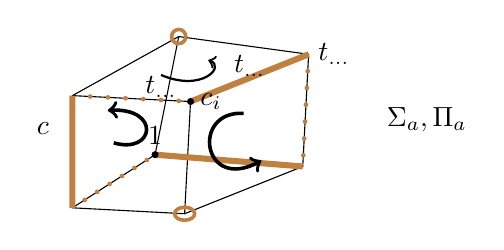
\begin{tikzpicture}[scale=.75]
\coordinate (a) at (0,2);\coordinate (b) at (2,1.9);
\coordinate (c) at (1.9,0);\coordinate (d) at (0,.1);
\coordinate (e) at (1.8,3);\coordinate (f) at (4,2.7);
\coordinate (g) at (3.9,.8);\coordinate (h) at (1.4,1);
\draw (a)--(b)--(c)--(d)--cycle;
\draw (e)--(f)--(g)--(h)--cycle;\draw (a)--(e) (b)--(f) (c)--(g) (d)--(h);
\draw[brown,line width=2.2pt] (a)--(d) (b)--(f) (h)--(g);
\foreach \u in {.15,.3,.45,.6,.75,.9}{
 \fill[brown] (\u*2,2-\u*.1) circle(.04);
 \fill[brown] (\u*1.4,.1+\u*.9) circle(.04);
 \fill[brown] (4-\u*.1,2.7-\u*1.9) circle(.04);}
\draw[brown,line width=1.3pt] (e) circle(.12);\draw[brown,line width=1.3pt] (c) ellipse(.17 and .11);
\fill (b) circle(.06);\fill (h) circle(.06);
\draw[->,thick] (1.5,2.35)..controls (2.2,2.05) and (2.6,2.5)..(2.3,2.6);
\draw[->,line width=1.3pt] (.7,1.2)..controls (1.4,1) and (1.5,1.8)..(.6,1.75);
\draw[->,line width=1.3pt] (2.9,1.7)..controls (2,1.75) and (2.2,.35)..(3.2,.9);
\node at (-.5,1.45) {$\unsure{c}$};\node[above] at (1.5,1.8) {$t_{\ldots}$};
\node[right] at (b) {$c_i$};\node[above] at (3,2.15) {$t_{\ldots}$};
\node[right] at (f) {$t_{\ldots}$};\node[above] at (h) {$1$};
\node at (6,1.6) {$\Sigma_a,\Pi_a$};
\end{tikzpicture}}
\[\deleted{\unsure{\tau}}\qquad\tau^2\]
\[\tau^{\unsure{8|\infty}}+\alpha_1\tau^7\;\text{---}\;+\alpha_8=0
\qquad\alpha_i\in\mathbb Z[b_{\cdot\cdot},c_\cdot,t_{\cdot\cdot}]\]
\[
\underbrace{b_s,c_s},t_s\ \big|\ \underbrace{t_a}\ \big|\ t_f
\]
\uline{Nb}
\[
\left\{\begin{aligned}b_s&=b_{s'}\\c_s&=c_{s'}\\t_a&=t_{a'}\end{aligned}\right.
\qquad\text{mais}\quad
\left\{\begin{aligned}
t_s&\ne t_{s'}&&\text{de degré }2\text{ sur }\unsure{A^{\mathfrak S_4}}\\
&&&\text{de degré }8\text{ sur }\unsure{A^{\mathfrak S_3}}\\
t_f&\ne t_{f'}&&\uline{\text{de degré }6\text{ sur }\unsure{B^{\mathfrak S_4}}}\\
&&&\text{de degré }8\ (?)\ \deleted{\unsure{4}}\text{ sur }A
\end{aligned}\right.
\]
\[
\begin{gathered}g\unsure{\tau|\bar\tau}\quad g'\tau\quad g''\tau\\
\sum g\tau\\\sum g\end{gathered}
\qquad
\begin{gathered}
\tau^{\unsure{8|\infty}}+\beta_1\tau^7\;\text{---}\;+\beta_8=0\\
\underbrace{(\alpha_1-\beta_1)}_{\gamma_1}\tau^7\;\text{---}\;+
 \underbrace{\alpha_8-\beta_8}=0
\end{gathered}
\]
\figure{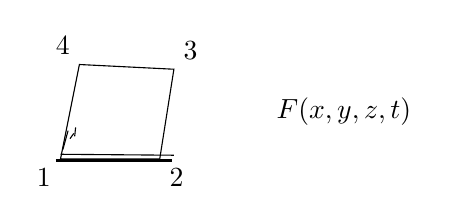
\begin{tikzpicture}[scale=.6]
\draw (0,0)--(.4,2)--(2.4,1.9)--(2.1,0)--cycle;
\draw[very thick] (-.1,-.03)--(2.35,-.03);\draw (0,.1)--(2.4,.08);
\draw (.05,.2)--(.16,.6);\draw (.2,.43)--(.28,.54);\draw (.3,.48)--(.32,.67);
\node[below left] at (0,0) {$1$};\node[below right] at (2.1,0) {$2$};
\node[above right] at (2.4,1.9) {$3$};\node[above left] at (.4,2) {$4$};
\node at (6,1) {$F(x,\uline{y,z},t)$};
\end{tikzpicture}}
\[H\subset\mathfrak S_4\]
\diagram{\begin{tikzcd}[ampersand replacement=\&]
B^H\arrow[d,dash,"\text{degré }6"]\\
B^{\mathfrak S_4}=B^G
\end{tikzcd}}
\[\alpha+\beta\tau\qquad a\quad b\quad\text{stables par}\quad\unsure{+}\mathfrak S_3^+\]
``
\[\alpha'+\beta'\tau'=\alpha'+\beta'(\sigma-\tau)
 =(\alpha'+\beta'\sigma)-\beta'\tau\]
\[\beta'=-\beta\;/\;\alpha'+\beta\sigma=\alpha\]
\[\alpha'=\alpha+\beta\sigma\;/\;(\alpha')'=\alpha=\alpha''\]
\margin{198}
\scanpage{200}
\diagram{\begin{tikzcd}[ampersand replacement=\&, column sep=large,row sep=large]
A \arrow[rr] \& {} \& B \arrow[d,dash,"3"]\\
A^{\mathfrak S_3^+} \arrow[u,"3"] \arrow[rr,dash,"2"] \& {} \& B_1=B^{\mathfrak S_3^+} \arrow[dd,dash,"2"]\\
{} \& B^{\mathfrak S_3}\arrow[ur,dash] \& {}\\
A^{\mathfrak S_3} \arrow[uu,"2"] \arrow[ur,dash] \arrow[rr,dash,"2"] \& {} \& B_0
\end{tikzcd}}
\[
\begin{aligned}
&\alpha+\beta\tau+\alpha'+\beta'\tau'\\
&=(\alpha+\alpha')+(\beta\tau+\beta'(\sigma-\tau))\\
&=\underbrace{\alpha+\alpha'}+\underbrace{\beta'\sigma}+(\beta-\beta')\tau
\end{aligned}
\]
\[\alpha+\alpha'+\beta\sigma-(\alpha+\alpha'+\beta'\sigma)
 =(\beta-\beta')\sigma\qquad\text{OK}\]

\mspage{L 22}
Tout ce que \unsure{je} croyais avoir à dire, à un moment ou à un autre\deleted{\unsure{d}}
de la réflexion, \inserted{(}que ce soit sur moi, ou sur tel autre, ou sur un milieu,
ou sur une époque, je l'ai dit, sans\inserted{jamais} avoir à bousculer mes réticences.
Il a suffi à chaque fois que je les examine avec attention, pour qu'elles s'évanouissent\deleted{\unsure{.}},
sans plus laisser de traces.
\margin{199}
\scanpage{201}
\[
\begin{aligned}\tau_f+\tau_{f'}&=\Sigma_a\\\tau_{f'}+\tau_{f''}&=\Sigma_{a'}\end{aligned}
\quad\longrightarrow\quad
\tau_f-\tau_{f''}=\Sigma_a-\Sigma_{a'}=\Sigma_{\bar a}-\Sigma_{\bar a'}
\]
i.e.\quad $\Sigma_a+\Sigma_{\bar a'}=\Sigma_{a'}+\Sigma_{\bar a}$

\figure{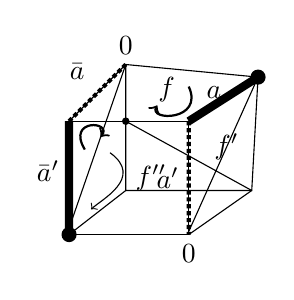
\begin{tikzpicture}[scale=.8]
\draw (0,1.8)--(1.9,1.8)--(1.9,0)--(0,0)--cycle;
\draw (.9,2.7)--(3,2.5)--(2.9,.7)--(.9,.7)--cycle;
\draw (0,1.8)--(.9,2.7) (1.9,1.8)--(3,2.5) (1.9,0)--(2.9,.7) (0,0)--(.9,.7);
\draw[line width=3pt] (0,0)--(0,1.8) (1.9,1.8)--(3,2.5);
\draw[densely dotted,line width=1.5pt] (0,1.8)--(.9,2.7) (1.9,1.8)--(1.9,0);
\draw (0,.1)--(.9,2.7) (1.9,.05)--(3,2.5) (.9,1.8)--(2.9,.7);
\fill (0,0) circle(.12);\fill (3,2.5) circle(.12);\fill (.9,1.8) circle(.06);
\node[above] at (.9,2.7) {$0$};\node[below] at (1.9,0) {$0$};
\node[above left] at (.4,2.3) {$\bar a$};\node[left] at (0,1) {$\bar a'$};
\node[above] at (2.3,2) {$a$};\node[left] at (1.9,.9) {$a'$};
\node at (1.55,2.3) {$f$};\node at (1.3,.9) {$f''$};\node at (2.5,1.4) {$f'$};
\draw[->,thick] (.25,1.35)..controls (-.05,1.85) and (.7,1.8)..(.5,1.55);
\draw[->,thick] (1.9,2.35)..controls (2.15,1.8) and (1.25,1.8)..(1.4,2.05);
\draw[->] (.65,1.3)..controls (1.2,.9) and (.5,.55)..(.35,.4);
\end{tikzpicture}}
\[\Sigma_a+\Sigma_{\bar a'}=\Sigma_{a'}+\Sigma_{\bar a}\]
\[4\cdot3\cdot2=24=48/2\]
\[
\begin{aligned}
\tau_f+\tau_{f'}&=\Sigma_a&\qquad
\tau_{\tilde f}+\tau_{\tilde f'}&=\Sigma_{\tilde a}=\Sigma_a\\
\tau_f\tau_{f'}&=\Pi_a&
\tau_{\tilde f}\tau_{\tilde f'}&=\Pi_{\tilde a}=\Pi_a
\end{aligned}
\]
donc $\{\tau_f,\tau_{f'}\}=\{\tau_{\tilde f},\tau_{\tilde f'}\}$

\figure{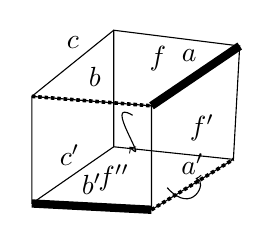
\begin{tikzpicture}[scale=.8]
\draw (0,1.8)--(1.9,1.65)--(1.9,0)--(0,.1)--cycle;
\draw (1.3,2.85)--(3.3,2.6)--(3.2,.8)--(1.3,1)--cycle;
\draw (0,1.8)--(1.3,2.85) (1.9,1.65)--(3.3,2.6) (1.9,0)--(3.2,.8) (0,.1)--(1.3,1);
\draw[line width=3pt] (1.9,1.65)--(3.3,2.6) (0,.1)--(1.9,0);
\draw[densely dotted,line width=1.3pt] (0,1.8)--(1.9,1.65) (1.9,0)--(3.2,.8);
\node[above] at (.65,2.4) {$c$};\node[above] at (1,1.8) {$b$};
\node[above] at (2.5,2.2) {$a$};\node[above] at (2.55,.4) {$a'$};
\node[above] at (.6,.55) {$c'$};\node[above] at (.95,.08) {$b'$};
\node at (2,2.4) {$f$};\node at (2.7,1.3) {$f'$};\node at (1.3,.5) {$f''$};
\draw[->] (1.6,1.5)..controls (1.1,1.8) and (1.9,.65)..(1.55,1);
\draw[->] (2.15,.35)..controls (2.55,-.1) and (2.8,.45)..(2.6,.5);
\end{tikzpicture}}
\[
\left.\begin{aligned}
\tau_f-\tau_{f''}&\unsure{=|-}\Sigma_a-\Sigma_{a'}=\Sigma_b-\Sigma_{b'}\\
\Sigma_a+\Sigma_{b'}&=\Sigma_b\unsure{\cdot|+}\Sigma_{a'}
\end{aligned}\right\}\quad\text{donc}\quad
\begin{gathered}\tau_f=\tau_{\tilde f}\quad\text{\textcircled{ou}}\\
\tau_f=\tau_{\tilde f'}\end{gathered}
\]
\figure{\begin{tikzpicture}\draw (0,0)--(6,.55);\end{tikzpicture}}
\[
\begin{aligned}
\Sigma_a-\Sigma_{a'}&=\Sigma_c-\Sigma_{c'}\\
\Sigma_a+\Sigma_{c'}&=\Sigma_c+\Sigma_{a'}
\end{aligned}
\]
$\Sigma_a$ ne dépend que de la direction de $a$

donc \uline{il n'y a que trois valeurs} de $\Sigma_a$

de même il n'y a que trois valeurs de $\Pi_a$

\figure{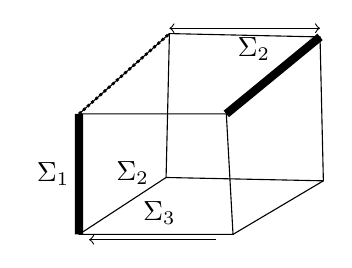
\begin{tikzpicture}[scale=.85]
\draw (0,1.8)--(2.2,1.8)--(2.3,0)--(0,0)--cycle;
\draw (1.35,3)--(3.6,2.95)--(3.65,.8)--(1.3,.85)--cycle;
\draw (0,1.8)--(1.35,3) (2.2,1.8)--(3.6,2.95) (2.3,0)--(3.65,.8) (0,0)--(1.3,.85);
\draw[line width=3pt] (0,0)--(0,1.8) (2.2,1.8)--(3.6,2.95);
\draw[densely dotted,line width=1pt] (0,1.8)--(1.35,3);
\draw[<->] (1.35,3.08)--(3.6,3.08);\draw[->] (2.05,-.08)--(.15,-.08);
\node[left] at (0,.9) {$\Sigma_1$};\node[above] at (.8,.6) {$\Sigma_2$};
\node[above left] at (3,2.45) {$\Sigma_2$};\node[above] at (1.2,0) {$\Sigma_3$};
\end{tikzpicture}}
$12$ relations de la forme $\Sigma_a+\Sigma_{a'}=\Sigma_b+\Sigma_{b'}$

\deleted{pour $\Sigma_a$ fixé}
Via opération du groupe symétrique $\mathfrak S_4$, elles se déduisent l'une de l'autre
\margin{200}
\scanpage{202}
\mspage{L 18}
présenter un tel travail, que ce soient \deleted{\unsure{des}}\inserted{les}
\inserted{manuels et autres} textes didactiques, \deleted{ou manuels,}
ou \deleted{\unsure{des}}\inserted{les} articles \deleted{\unsure{ou}}\inserted{et}
mémoires\deleted{\unsure{,}} \deleted{\unsure{ou de}} originaux, ou les \deleted{exposés} cours oraux
\deleted{ou}\inserted{et} exposés de séminaires etc.
Il y a, depuis des millénaires semblerait-il, depuis les\deleted{ori} origines mêmes de\deleted{\unsure{s}}
la mathématique et des autres sciences, \deleted{que nous cultivons,}
une sorte de ``conspiration du silence'' autour de ces \deleted{aspect}
``\uline{inavouables} \uline{labeurs}'' qui préludent à l'éclosion de toute idée nouvelle,
grande ou petite, venant renouveler notre connaissance d'une portion de\inserted{ce} monde où nous vivons.

Pour tout dire, il semblerait que la répression de la connaissance de cet aspect là\deleted{, de plus}
ou de ce stade-là, le plus crucial de tous\deleted{\unsure{,}} dans le travail de découverte
(et dans le travail créateur en général), soit à tel point efficace, à tel point intériorisé
par ceux-là même qui pourtant connaissent un tel travail de première main, qu'on jurerait souvent
que même ceux-là \deleted{l'ont oublié} en ont éradiqué toute trace de leur souvenir conscient.
Un peu comme dans une société puritaine à outrance, une femme aurait éradiqué de son souvenir,
\deleted{toute trace} en relation à\inserted{chacun de} ces enfants qu'elle se fait un devoir de moucher
et de torcher, le moment de l'étreinte (subie peut-être à contre-coeur) qui le\deleted{\unsure{s}} fit concevoir,
les longs mois de la grossesse\deleted{\unsure{,}} (vécue comme\inserted{une} \unsure{inconvenante})
et les longues heures de l'accouchement (vécues comme un\inserted{peu ragoûtant} martyre,
suivi enfin d'une délivrance).
\margin{\figure{\begin{tikzpicture}[scale=.3]
\draw[blue,->] (0,0)--(2,0)--(2,1.5)--(5,1.5);\draw[blue] (1.8,0)--(1.8,1.5);
\end{tikzpicture}}}
Cette comparaison peut paraître \unsure{outée|outrée}, et elle l'est peut-être,
si je l'applique à ce que je me rappelle à présent de l'esprit que j'ai connu dans le milieu\inserted{mathématique}
dont je faisais moi-même partie, il y a encore vingt ans.
Mais \deleted{dans} j'ai pu me rendre compte, au cours de ma réflexion\deleted{, \unsure{que dans les}}
dans Récoltes et Semailles, et de façon saisissante ces tout derniers mois surtout
(avec l'écriture des Quatre Opérations), qu'il y a eu depuis mon départ de la scène mathématique
une \deleted{dégra} dégradation stupéfiante dans l'esprit qui aujourd'hui fait loi dans les milieux
que j'avais connus, et (me semble-t-il, dans une large mesure au moins) dans le monde mathématique en général.
Il est possible même que mon départ, tant par ma personnalité mathématique très particulière
que par les conditions qui ont entouré ce départ, ait agi comme un catalyseur dans une évolution
qui était déjà en train de se faire ($\unsure{*|x}$); \deleted{\unsure{et}}\inserted{évolution}
dont bien sûr je n'ai rien su percevoir (pas plus qu'aucun de mes collègues et amis,
à la seule exception peut-être de Claude Chevalley).
L'aspect de cette dégradation\inserted{(parmi de nombreux autres ($\unsure{**|xx}$))}
auquel je pense ici est le \deleted{\unsure{dérision ou mépris}}
m\,é\,p\,r\,i\,s\quad t\,a\,c\,i\,t\,e,
\deleted{prenant parfois des formes} quand ce n'est la dérision
\deleted{à peine voilée}\inserted{sans équivoque}, vis à vis de ce qui, dans le travail (mathémati-
\margin{201}
\scanpage{203}
\figure{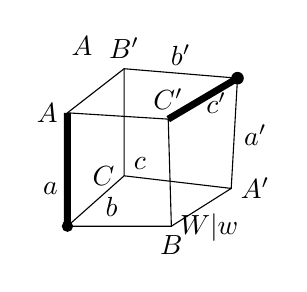
\begin{tikzpicture}[scale=.8]
\draw (0,1.8)--(1.6,1.7)--(1.65,0)--(0,0)--cycle;
\draw (.9,2.5)--(2.7,2.35)--(2.6,.6)--(.9,.8)--cycle;
\draw (0,1.8)--(.9,2.5) (1.6,1.7)--(2.7,2.35) (1.65,0)--(2.6,.6) (0,0)--(.9,.8);
\draw[line width=2.5pt] (0,0)--(0,1.8) (1.6,1.7)--(2.7,2.35);
\fill (0,0) circle(.09);\fill (2.7,2.35) circle(.1);
\node[left] at (0,1.8) {$A$};\node[left] at (0,.6) {$a$};
\node[above] at (.7,0) {$b$};\node[below] at (1.65,0) {$B$};
\node[right] at (2.6,.6) {$A'$};\node[right] at (2.65,1.45) {$a'$};
\node[above] at (1.8,2.4) {$b'$};\node[above] at (.9,2.5) {$B'$};
\node[above left] at (.55,2.55) {$\deleted{\unsure{A}}$};
\node[above] at (1.6,1.7) {$C'$};\node[right] at (2.05,1.95) {$c'$};
\node[left] at (.9,.8) {$C$};\node[above] at (1.15,.75) {$c$};
\node[below] at (2.25,.35) {$\unsure{W|w}$};
\end{tikzpicture}}
\margin{\figure{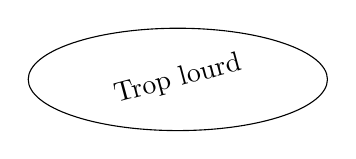
\begin{tikzpicture}\draw (0,0) ellipse (1.9 and .65);
\node[rotate=15] at (0,0) {Trop lourd};\end{tikzpicture}}}
\[
\begin{gathered}
\Sigma_a\quad\Sigma_b\quad\Sigma_c\quad\Sigma_{AB'}\quad
\unsure{\Sigma_{BA'}|\Sigma_{BC'}}\quad\Sigma_{CB'}\quad\Sigma_{CA'}\quad\Sigma_{AC'}\\
\Sigma_{a'}\quad\Sigma_{b'}\quad\Sigma_{c'}
\end{gathered}
\]
\figure{\begin{tikzpicture}
\node[anchor=north west,inner sep=0] at (0,0) {\diagram{\begin{tikzcd}[ampersand replacement=\&, row sep=.6em,column sep=large]
\Sigma_a+\Sigma_{c'}=\Sigma_{AB'}+\Sigma_{BC'}\\
\Sigma_a+\Sigma_{b'}=\Sigma_{AC'}+\Sigma_{CB'}\\
\Sigma_b+\Sigma_{a'}=\Sigma_{BC'}+\Sigma_{CA'}\\
\Sigma_b+\Sigma_{c'}=\Sigma_{BA'}+\Sigma_{AC'}\\
\Sigma_c+\Sigma_{b'}=\Sigma_{CA'}+\Sigma_{AB'}\\
\Sigma_c+\Sigma_{a'}=\Sigma_{CB'}+\Sigma_{BA'}\\[.8em]
\Sigma_a+\Sigma_{CA'}=\Sigma_b+\Sigma_{CB'}\ .\\
\Sigma_{a'}+\Sigma_{AC'}=\Sigma_{b'}+\Sigma_{BC'}\\
\Sigma_b+\Sigma_{AB'}=\Sigma_c+\Sigma_{AC'}\ .\\
\Sigma_{b'}+\Sigma_{BA'}=\Sigma_{c'}+\Sigma_{CA'}\\[.6em]
\Sigma_c+\Sigma_{BC'}=\Sigma_a+\Sigma_{BA'}\ .\\
\Sigma_{c'}+\Sigma_{CB'}=\Sigma_{a'}+\Sigma_{AB'}
\end{tikzcd}}};
\draw (8.0,-.05)..controls (8.25,-.6) and (8.1,-1.0)..(7.8,-1.45)
 ..controls (8.35,-1.9) and (8.3,-2.45)..(7.9,-2.9);
\draw (7.85,-.7)..controls (8.65,-1.2) and (8.55,-1.8)..(7.85,-2.15)
 ..controls (8.8,-2.65) and (8.6,-3.4)..(8.05,-3.55);
\draw (-.25,-.15)..controls (-.15,-2) and (-.05,-3.8)..(-.55,-4.1)
 ..controls (-.05,-4.25) and (-.15,-6.5)..(-.1,-8.65);
\draw[very thick] (.15,-4.55)--(-.02,-4.55)--(-.02,-7.2)--(.15,-7.2);
\end{tikzpicture}}
\margin{$\exists\sigma$ avec
\[\sigma_{\uline{a}}+\sigma_{\uline{b}}+\sigma_{\uline{c}}=\sigma\]
$\forall$ triples d'arêtes formant un ``demi hexagone''
\figure{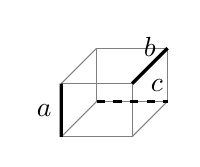
\begin{tikzpicture}[scale=.45]
\draw[gray] (0,0)--(0,1.5)--(2,1.5)--(2,0)--cycle;
\draw[gray] (1,1)--(1,2.5)--(3,2.5)--(3,1)--cycle;
\draw[gray] (0,0)--(1,1) (0,1.5)--(1,2.5) (2,1.5)--(3,2.5) (2,0)--(3,1);
\draw[very thick] (0,0)--(0,1.5) (2,1.5)--(3,2.5);
\draw[dashed,very thick] (1,1)--(3,1);
\node[left] at (0,.75) {$\uline{a}$};\node[above] at (2.5,2) {$\uline{b}$};
\node[above] at (2.7,1) {$\uline{c}$};\end{tikzpicture}}
\[\Sigma_{a'}+\Sigma_{AC'}=\Sigma_{b'}+\Sigma_{BC'}\]}
\margin{chacune des six dernières relations est conséquence des cinq autres,
comme on voit en sommant, \unsure{qui|que} donne $0=0$ !}
\[
\begin{aligned}
&3(\Sigma_a\unsure{+|-}\Sigma_b\unsure{+|-}\Sigma_c+\Sigma_{a'}
 \unsure{+|-}\Sigma_{b'}+\Sigma_{c'})
 +(\Sigma_{CA'}+\Sigma_{AC'}\;\text{---}\;\text{---})\\
&=(\Sigma_a+\Sigma_b\unsure{+|-}\Sigma_c\unsure{+|-}\Sigma_{a'}
 \unsure{+|-}\Sigma_{b'}\unsure{+|-}\Sigma_{c'})+3(\Sigma_{CA'}+\Sigma_{AC'})
\end{aligned}
\]
\margin{202}
\scanpage{204}
\mspage{L 17}
entrevu seulement et encore moins vu et touché, \deleted{pour} peu à peu se
\deleted{dégager de son manteau \inserted{\deleted{d'ombre et}} de brumes, et se}
décante\deleted{r} de l'impondérable, se dégage\deleted{r} de son manteau d'ombre et de brumes
\deleted{et}\inserted{pour} prendre forme et chair\inserted{et poids}\inserted{\ldots}
\margin{\figure{\begin{tikzpicture}[scale=.3]
\draw[blue] (0,0)--(1,0)--(1,1)--(2.5,1);\draw[blue] (.9,0)--(.9,.9);
\end{tikzpicture}}}

\inserted{\figure{\begin{tikzpicture}[scale=.25]\draw[blue] (0,0)--(.8,0)--(.8,1)--(2,1);\draw[blue] (.65,0)--(.65,1);\end{tikzpicture}}}\deleted{Ce sont}\inserted{C'est}\deleted{ces stades}\inserted{cette partie-}là du travail,
de piètre apparence pour ne pas dire\inserted{(bien des fois)} foireux, qui
\deleted{\unsure{en représentent aussi les points}}\inserted{en \deleted{sont} est aussi la \deleted{plus}}
\deleted{névralgique}\inserted{partie la plus délicate et la plus essentielle}
--- celle où, véritablement quelque chose de n\,o\,u\,v\,e\,a\,u fait son apparition,
par l'effet d'une attention intense, d'une sollicitude, d'un respect pour cette chose fragile,
infiniment délicate, sur le point de naître. C'est la partie créatrice entre toutes ---
celle\deleted{s} de la conception et d\deleted{e la}\inserted{'une}\inserted{lente} gestation
\deleted{d'un fragile embryon} dans les chaudes ténèbres de la matrice nourricière,
\deleted{\unsure{évoluant en silence}} depuis l'invisible double gamète \deleted{initiale}
originelle devenant\inserted{informe} embryon et se transformant au fil des jours et des mois,
par un travail obscur et intense, invisible et sans apparence, en un nouvel être en chair et en os.

C'est là aussi la partie\inserted{éminemment} ``yin'', ``féminine\deleted{\unsure{,}}'' du travail de découverte\inserted{.}\deleted{---}
\deleted{alors que \deleted{la partie}}\deleted{l'}\inserted{L'}aspect complémentaire ``yang'', ou masculin,
s'apparenterait plutôt \deleted{aux} au travail à coups de marteaux ou de masse,
sur un burin bien affûté ou sur un coin de bon acier trempé.
L'un et l'autre aspect a sa raison d'être et sa fonction, en symbiose inséparable\inserted{l'un}
avec l'autre --- ou pour mieux dire, ce sont là l'\uline{épouse} et \uline{l'époux}
du couple des deux forces cosmiques originelles, dont l'étreinte
\inserted{\deleted{sans cesse}}\deleted{renouvelée fait}
sans cesse renouvelée fait resurgir sans cesse les obscurs labeurs créateurs de la conception,
de la gestation et de la naissance --- de la naissance de l'\,e\,n\,f\,a\,n\,t, de la chose nouvelle.

La deuxième chose sur laquelle je sentais le besoin de m'exprimer, dans ma fameuse ``introduction''
\deleted{philosophique et} personnelle et ``philosophique'' à un texte mathématique,
c'était au sujet de la nature du travail créateur justement.
Je me rendais compte, depuis des années, que cette nature était généralement ignorée,
occultée par des clichés à tout venant et par des\inserted{répressions et des} peurs ancestrales.
A quel point il en est bien ainsi, je l'ai découvert\inserted{\unsure{après seulement,|alors seulement,}}
progressivement, en fil des jours et des mois, tout au cours de la réflexion et de ``l'enquête''
poursuivie dans Récoltes et Semailles.
C'est dès les tout débuts de cette réflexion, au mois de juin 1983, que je suis saisi pour la première fois
(pour l'oublier\inserted{un peu} par la suite\deleted{\ldots) par}
\inserted{, sous le flux des découvertes imprévues\ldots) par}
la portée de ce fait d'anodine apparence, et pourtant \unsure{asses|assez} stupéfiant,
pour peu seulement qu'on s'y arrête tant soit peu: que cette partie ``créatrice entre toutes''
dont je viens de parler dans le travail de découverte,
\uline{ne transparaît pratiquement nulle part} dans les textes\inserted{ou discours} qui sont censés
\margin{203}
\scanpage{205}

\figure{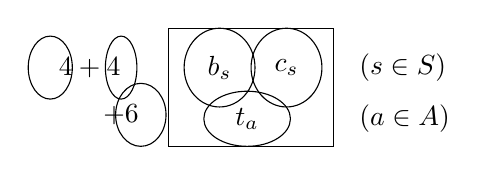
\begin{tikzpicture}
\node at (0,0) {$4+4$};\node at (.4,-.6) {$+6$};
\draw (-.5,0) ellipse(.28 and .4);\draw (.4,0) ellipse(.2 and .4);\draw (.65,-.6) ellipse(.32 and .4);
\draw (1,-1)--(1, .5)--(3.1,.5)--(3.1,-1)--cycle;
\node at (1.65,0) {$b_s$};\node at (2.5,0) {$c_s$};\node at (2,-.65) {$t_a$};
\draw (1.65,0) ellipse(.45 and .5);\draw (2.5,0) ellipse(.45 and .5);\draw (2,-.65) ellipse(.55 and .35);
\node[right] at (3.3,0) {$(s\in S)$};\node[right] at (3.3,-.65) {$(a\in A)$};
\end{tikzpicture}}
avec $b_s=b_{\bar s}$, $c_s=c_{\bar s}$, $\unsure{b_a|t_a}=t_{\bar a}$.

\figure{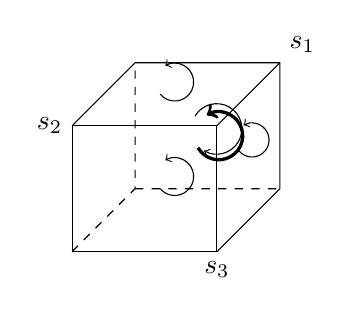
\begin{tikzpicture}[scale=.8]
\draw (0,0)--(0,2)--(2.3,2)--(2.3,0)--cycle;
\draw (0,2)--(1,3)--(3.3,3)--(3.3,1)--(2.3,0) (2.3,2)--(3.3,3);
\draw[dashed] (0,0)--(1,1)--(1,3) (1,1)--(3.3,1);
\node[above right] at (3.3,3) {$s_1$};\node[left] at (0,2) {$s_2$};\node[below] at (2.3,0) {$s_3$};
\draw[->] (1.4,2.5) arc(220:480:.3);
\draw[->] (1.4,1) arc(220:480:.3);
\draw[->] (2.65,1.6) arc(220:480:.27);
\draw[->] (1.95,2.15) arc(150:-120:.4);
\draw[->,very thick] (2,1.65) arc(210:480:.38);
\end{tikzpicture}}
Si $\delta(s)\inserted{\in I}$ est la diagonale qui passe par $s$, on a
\[b_s=\operatorname{Tr}X_s\qquad c_s=\det X_s\]
Si $\delta(a)\in\unsure{\mathcal P|P}_2(I)$ est l'une des deux diagonales qui passent par les
\deleted{\unsure{sommets}} de $a$, on a
\[t_a=\operatorname{Tr}X_iX_j\inserted{=\operatorname{Tr}X_jX_i}
\quad\text{si }\delta(a)=\{i,j\}\]

\figure{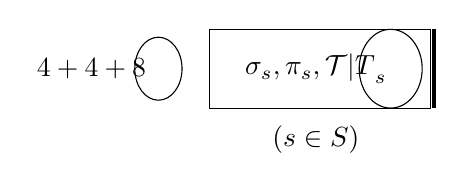
\begin{tikzpicture}
\node at (0,0) {$4+4+8$};\draw (.85,0) ellipse(.3 and .4);
\draw (1.5,-.5) rectangle (4.3,.5);\draw[very thick] (4.35,-.5)--(4.35,.5);
\node at (2.85,0) {$\sigma_s,\pi_s,\unsure{\mathcal T|T}_s$};\draw (3.8,0) ellipse(.4 and .5);
\node at (2.85,-.9) {$(s\in S)$};\end{tikzpicture}}
$s$ correspond à un triple $(i,j,k)$ à perm. circulaire près
\[\begin{aligned}
\mathcal T_s&=\operatorname{Tr}X_iX_jX_k
 =\operatorname{Tr}X_{\deleted{\unsure{i}}\inserted{j}}X_kX_i
 =\operatorname{Tr}X_kX_iX_j\\
\mathcal T_{\bar s}&=\operatorname{Tr}X_kX_jX_i
 =\operatorname{Tr}X_jX_iX_k=\operatorname{Tr}X_iX_kX_j .
\end{aligned}\]

\figure{\begin{tikzpicture}
\node[draw,ellipse] at (0,0) {$4+4$ relations};
\node at (2.2,0) {$(R_s)$};\node at (2.2,-.5) {$\underbrace{\phantom{R_s}}_{R_{\bar s}}$};
\node[draw,rectangle] at (5,0) {$\begin{aligned}
\sigma_s&=\sigma_{\bar s}=\mathcal T_s+\mathcal T_{\bar s}\\
\pi_s&=\unsure{\pi_{\bar s}|\sigma_{\bar s}}=\mathcal T_s\cdot\mathcal T_{\bar s}
\end{aligned}$};\end{tikzpicture}}
\[\begin{aligned}
\sigma_s=\sigma_{\bar s}&=b_it_{jk}+b_jt_{ki}+b_kt_{ij}-b_ib_jb_k\\
\deleted{\unsure{\sigma_s}}&=b_{s_1}t_{ss_1}+b_{s_2}\unsure{b_{ss_2}|t_{ss_2}}+b_{s_3}t_{ss_3}-b_{s_1}b_{s_2}b_{s_3}
\end{aligned}\]
où $s_1,s_2,s_3$ sont les sommets adjacents à $s$
\[\left\{\begin{aligned}
\pi_s=\pi_{\bar s}={}&t_{ss_1}t_{ss_2}t_{ss_3}
 +\deleted{(c_{s_1}t_{ss_1}^{\unsure{2}}+c_{s_2}t_{ss_2}^{\unsure{2}}+c_{s_3}t_{ss_3}^{\unsure{2}})}\\
&\inserted{+\bigl[c_{s_1}t_{ss_1}(t_{ss_1}-b_{s_2}b_{s_3})
 +c_{s_2}t_{ss_2}(t_{ss_2}-b_{s_3}b_{s_1})
 +c_{s_3}t_{ss_3}(t_{ss_3}-b_{s_1}b_{s_2})\bigr]}\\
&+(\unsure{b_{ss_1}^{2}|b_{s_1}^{2}}c_{ss_2}c_{ss_3}
 +\unsure{b_{ss_2}^{2}|b_{s_2}^{2}}c_{ss_3}c_{ss_1}
 +\unsure{b_{ss_3}^{2}|b_{s_3}^{2}}c_{ss_1}c_{ss_2})
\end{aligned}\right.\]

\figure{\begin{tikzpicture}
\node[draw,ellipse] at (0,0) {$6$};
\draw (1,-1.2)--(1,.5)--(2.1,.5)--(2.1,-.4)--(2.8,-.4)--(2.8,-1.2)--cycle;
\node[draw,ellipse] at (1.6,0) {$\mathcal T_f$};\node at (1.9,-.9) {$\sigma_a,\pi_a$};
\node[right] at (2.5,0) {$(f\in F)$};\node[right] at (3,-.9) {$(a\in A)$};\end{tikzpicture}}
Si $f$ correspond à la permutation circulaire $(i,j,k,l)$ de $I$, on a
\[\mathcal T_f=\operatorname{Tr}X_iX_jX_kX_l
 =\deleted{\unsure{\mathcal T_f=}}\operatorname{Tr}X_jX_kX_lX_i
 =\operatorname{Tr}X_kX_lX_iX_j=\operatorname{Tr}X_lX_iX_jX_k\]
Si $f,f'$ sont adjacentes le long d'une arête $a=(s,t)$

\figure{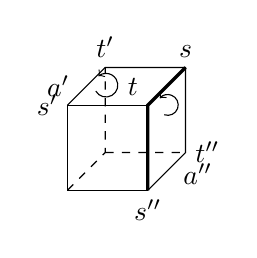
\begin{tikzpicture}[scale=.6]
\draw (0,0)--(0,1.8)--(1.7,1.8)--(1.7,0)--cycle;
\draw (0,1.8)--(.8,2.6)--(2.5,2.6)--(2.5,.8)--(1.7,0) (1.7,1.8)--(2.5,2.6);
\draw[dashed] (0,0)--(.8,.8)--(.8,2.6) (.8,.8)--(2.5,.8);
\draw[very thick] (1.7,0)--(1.7,1.8)--(2.5,2.6);
\node[above] at (2.5,2.6) {$s$};\node[above left] at (1.7,1.8) {$t$};
\node[left] at (0,1.8) {$s'$};\node[above] at (.8,2.6) {$t'$};
\node[below] at (1.7,0) {$s''$};\node[right] at (2.5,.8) {$t''$};
\node[right] at (2.25,.35) {$a''$};\node[left] at (.25,2.2) {$a'$};
\draw[->] (.6,2.1) arc(210:490:.25);\draw[->] (2.05,1.6) arc(250:500:.22);
\end{tikzpicture}}

\diagram{\begin{tikzcd}[ampersand replacement=\&, row sep=small,column sep=small]
f=(s,\arrow[d]\&t,\arrow[d]\&s'',\arrow[d]\&t'')\arrow[d]\&\quad f'=(t,\arrow[d]\&s,\arrow[d]\&t'',\arrow[d]\&s'')\arrow[d]\\
i\&j\&k\&l\&j\&i\&k\&l
\end{tikzcd}}
\deleted{\unsure{NB}} d'où
\[\mathcal T_f=\operatorname{Tr}X_iX_j(X_kX_l),\quad
\mathcal T_{f'}=\operatorname{Tr}X_jX_i(X_kX_l),\quad\text{on a}\]
\margin{204}
\scanpage{207}
\figure{\begin{tikzpicture}
\node[draw,ellipse] at (0,0) {$R_a$};
\node[align=left] at (0,-1) {$12+12$\\relations};
\node[draw,rectangle] at (3.1,0) {$\begin{aligned}
\mathcal T_f+\mathcal T_{f'}&=\sigma_a\\
\mathcal T_f\mathcal T_{f'}&=\pi_a
\end{aligned}$};\end{tikzpicture}}
avec
\[\begin{aligned}
\sigma_a={}&\operatorname{Tr}X_kX_l\operatorname{Tr}X_iX_j
 +\operatorname{Tr}X_i\operatorname{Tr}X_jX_kX_l
 +\operatorname{Tr}X_j\operatorname{Tr}X_kX_lX_i\\
&-\operatorname{Tr}X_i\operatorname{Tr}X_j\operatorname{Tr}X_kX_l\\
&\deleted{=\unsure{t_s+t}}\\
={}&\underbrace{\unsure{t_{a'a''}|t_{a''}}}_{\unsure{t_{a''}}}t_a
 +b_s\mathcal T_s+b_t\mathcal T_t-b_sb_t t_{a'a''}
\end{aligned}\]
\figure{\begin{tikzpicture}
\draw (0,0)..controls(.6,-.5) and (1,-.9)..(1.1,-1.5);\end{tikzpicture}}
\[\pi_a=\text{---}\]
expression \deleted{plus}\inserted{un peu} compliquée en
\[\begin{gathered}
\deleted{\operatorname{Tr}X_i,\unsure{d}}\quad b_i,c_i,b_j,c_j,t_{kl},c_kc_l\\
t_{ij}\quad\underbrace{\mathcal T_{jkl}}_{\mathcal T_s}\quad
\underbrace{\mathcal T_{kli}}_{\mathcal T_t}
\end{gathered}\]
\[
28\text{ variables}\quad
\begin{array}{ccccc}
\multicolumn{3}{c}{\overbrace{\phantom{4\quad4\quad6}}^{14}}&
\multicolumn{2}{c}{\overbrace{\phantom{8\quad6}}^{14}}\\[-.6em]
4&4&6&8&6\\
b_s&c_s&t_a,&\mathcal T_s,&\mathcal T_f
\end{array}
\]
$32$ relations !
\margin{206}
\scanpage{208}
\margin{447}
(*\deleted{*}) Les deux autres livres sont les thèses de Jean Giraud et de \deleted{Monique} Monique Hakim (sur le formalisme des champs et de la 1-cohomologie non commutative, et sur les schémas relatifs sur des topos annelés généraux).

\margin{448}
(*) Cette citation (traduite) est extraite de la courte lettre (adressée au Dr. Peters) du 18 février l'an dernier, où je l'informais de ma décision de me retirer de l'``editorial board'' des Grundlehren. Le Dr. Peters avait en fait quitté déjà le Springer Verlag (il travaille à présent dans le Birkhäuser Verlag), et la correspondance s'est continuée avec le \deleted{Dr.} Dr. J. Heinze, en charge des Grundlehren dans la maison Springer\deleted{ Verlag}. J'avais demandé\deleted{e} qu'une copie de ma lettre soit envoyée à chacun des co-éditeurs des Grundlehren (au nombre de dix-huit), et avais réitéré cette prière\deleted{,} au Dr Heinze\deleted{,} à deux reprises (en avril 84 et janvier 85) sans qu'il juge utile de me \deleted{dire} préciser si oui ou non elle avait été respectée (il \inserted{est} appar\deleted{aît}\inserted{\unsure{u}} que \uline{non}). J'ai pris la peine d'envoyer moi-même une copie de \unsure{ma|la} lettre \deleted{de démission, avec quelques mots d'explication,} à chacun des dix-huit éditeurs, avec quelques mots d'explication \deleted{\unsure{adressé}} au sujet de cet envoi. \deleted{\unsure{Parmi ces éditeurs j'en conn}}\inserted{Je} connais bien personnellement sept \unsure{parmi} \deleted{ces éditeurs,}\inserted{eux,} et \deleted{cinq entre eux} \deleted{je}\inserted{j'en} comptais\inserted{cinq} parmi mes amis. Un seul \deleted{\unsure{k}} (Artin) a pris la peine de me répondre, et aucun apparemment \unsure{n}\deleted{\unsure{e}}\inserted{\unsure{'a}} rien trouvé d'anormal \deleted{\unsure{visà}} (ne serait-ce que vis-à-vis de \unsure{l\,u\,i\,-\,m\,ê\deleted{\unsure{e}}\,m\,e}) que la maison Springer n'ait pas\inserted{elle-même} pris la peine de lui faire parvenir \deleted{elle-même} \deleted{au mois} (et dès le mois de février 1984) la lettre en question.

(**\deleted{*}) Ce sont les volumes n\textsuperscript{os} 288,340, 569, 589, 900.

(***\deleted{*}) Comme je le précise dans l'avant-dernière note de b. de p., le Dr. Peters a depuis quitté\inserted{le} Springer Verlag pour Birkhäuser Verlag.

\margin{450}
(*) \deleted{Voir mes observations\inserted{\deleted{(p. \unsure{899})}} dans la sous-note ``Les double-sens -- ou l'art de l'arnaque'' (n° $\unsure{169_7|169_2}$), concernant} \inserted{Dans} le fameux ``Fil d'Ariane'' \deleted{\unsure{à travers SGA}}\inserted{(à travers SGA 4 etc)} dans le volume nommé `` SGA $4\frac12$ '', \deleted{\unsure{où}} rien ne pourrait laisser supposer au lecteur que j'aie eu l'honneur de faire des exposés dans SGA 4 et SGA 5 (par contre, j'ai\inserted{bien} eu celui de ``collaborer'' à ``SGA $4\frac12$ '' ...).
\inserted{Voir à ce sujet mes observations dans la note ``Les double-sens -- ou l'art de l'arnaque'' (n° $\unsure{169_2|167_2}$), p. 899.}

\margin{\unsure{452|451}}
(*) J'ai songé d'ailleurs aussi qu'il se pourrait bien que la situation se renverse, et que ce soit l'estimable entreprise qui m'intente un procès, pour atteinte à sa réputation. \deleted{J'imagine que} \deleted{c}\inserted{C}es gens ``au service de la \deleted{s}\inserted{S}cience'', ils doivent être pointilleux sur ce chapitre \deleted{\unsure{--}} \inserted{(}du moment que c'est de \uline{leur} \deleted{propre} réputation qu'il s'agit ...\inserted{)}.

\margin{452}
(*) Cette idée-force de bâtir des ``maisons'', et qui soient bonnes ``pour tous'', a joué un rôle considérable dans mon oeuvre mathématique, et ceci depuis le début des années cinquante déjà. Cela a été l'expression \unsure{concrète} \deleted{de \unsure{la pulsion de}}\inserted{dans mon travail de} ce que j'ai appelé la ``pulsion de service'' \deleted{en moi}, qui a fait partie (sans même que je la décèle avant la réflexion ``La clef du yin et du yang'') des \deleted{\unsure{motivations profon}} forces profondes donnant leur force \unsure{vive} à mon travail mathématique. L'archétype de la ``maison'' apparaît pour la première fois dans ma réflexion, \deleted{et avec} sans que je\inserted{ne} l'aie \deleted{\unsure{entrev}} \unsure{pressenti}, et avec une grande force, dans la note\inserted{(du 26 novembre)} ``Yin le serviteur, et les nouveaux maîtres'' (n° 135).
\margin{207}
\scanpage{209}

\figure{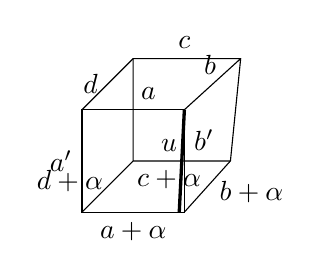
\begin{tikzpicture}[scale=.65]
\draw (0,0)--(0,2)--(2,2)--(2,0)--cycle;
\draw (0,2)--(1,3)--(3.1,3)--(2.9,1)--(2,0) (2,2)--(3.1,3);
\draw (0,0)--(1,1)--(1,3) (1,1)--(2.9,1);
\draw[very thick] (1.9,0)--(2,2);
\node[above] at (1.3,2) {$a$};\node[above] at (2.5,2.5) {$b$};
\node[above] at (2,3) {$c$};\node[left] at (.5,2.5) {$d$};
\node[left] at (0,1) {$a'$};\node[right] at (2,1.4) {$\unsure{b'}$};
\node[below] at (1,0) {$a+\alpha$};\node[right] at (2.5,.4) {$b+\alpha$};
\node[below] at (1.7,1) {$c+\alpha$};\node[left] at (.6,.6) {$d+\alpha$};
\node[above] at (1.7,1) {$\deleted{\unsure{u}}$};
\end{tikzpicture}}

\figure{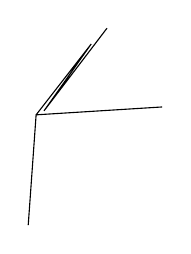
\begin{tikzpicture}
\draw (0,-1.4)--(.1,0)--(1.7,.1);
\draw (.1,0)--(.8,.9)--(.2,.05)--(1,1.1);\end{tikzpicture}}

\figure{\begin{tikzpicture}[scale=1.1]
\draw (0,0)--(0,3);\draw[->] (0,3)--(3.8,3.15);
\draw (3.8,2.95)--(3.65,.1) (0,-.1)--(3.7,-.1);
\draw (0,3.15)--(1.8,4.6) (1.9,4.75)--(5.8,4.95)--(5.45,1.4);
\draw (3.9,3.2)--(5.8,4.95) (3.85,-.1)--(5.5,1.25);
\draw (2,1.25)--(5.3,1.35) (.1,0)--(.9,.55) (1.65,1.5)--(1.65,2.15);
\node[draw,ellipse] at (2.4,3.3) {$a$};\node[draw,ellipse] at (4.55,4) {$b$};
\node[draw,ellipse] at (3.75,5.12) {$c$};\node[draw,ellipse] at (.55,4.05) {$d$};
\node[draw,ellipse] at (-.3,1.2) {$u$};
\node[right] at (3.8,1.55) {$v=u\unsure{-|\cdot}(d-b)$};
\node[right,rotate=12] at (5.65,2.65) {$v+(c-a)=u-(d-b)+(c-a)$};
\node[above] at (1.65,2.3) {$u+c-a$};
\node[above] at (2.7,1.3) {$c+\alpha$};\node[right] at (4.5,.6) {$b+\alpha$};
\node[above] at (.75,.7) {$d+\alpha$};\node[above] at (2.2,-.1) {$a+\alpha\to$};
\node[draw,ellipse] at (2.8,.1) {$\unsure{a'|a''}$};
\end{tikzpicture}}
\[\boxed{d-b=u-v}=d-b\unsure{-=|=}u-v\]
i.e.
\[d+v=b+u\]
\[d-u=b-v\]
\[
a,b,c,d,\underset{\substack{|\\\text{ou }a+\alpha=\unsure{a^!|a'}}}{\alpha},u
\]
\margin{208}
\scanpage{210}
\mspage{452}
années à vivre -- le temps passe vit\deleted{\unsure{t}}e, et je vois plein de choses passionantes à faire dans ce temps qui me reste. Ça \deleted{\unsure{ne}} doit pas être bien passionant de réunir des pièces à conviction pour convaincre des juges que j'ai quelque chose à voir avec les SGA. Ce n'est pas pour eux, pas plus que pour Monsieur K.F. Springer, que je me suis fatigué à les \unsure{édrire|écrire} ...

Quant à ceux (à part moi-même) pour qui j'ai écrit les SGA, la relation qu'ils entretiennent à ce qui (pour moi en tous cas) reste une part de moi-même, ne m'est nullement indifférente. Elle fait partie de leur relation à ma personne. Chose étrange, je ne connais bien cette relation (ou du moins, tant soit peu) que pour mes cinq élèves cohomologistes: ceux-là même grâce auxquels il est devenu possible aujourd'hui \deleted{\unsure{qu'un Dr. K.F}} à un Dr. K.F. Springer de m'envoyer \unsure{balàder|balader}, comme un \deleted{fanfaron}\inserted{malpropre} qui n'aurait rien à dire sur ce qu'on fait ou ne fait pas avec des\inserted{ }textes portant le sigle SGA, que le quidam en question figure ou non sur\deleted{\unsure{à}} la couverture.

Le lecteur mathématicien qui m'aurait suivi jusqu'ici, et qui aurait un jour hanté les SGA (les vrais, j'entends)\deleted{\unsure{*}}, peut-être qu'il aura idée de me toucher un mot sur ce qu'il en pense lui-même. C'est sûr que ça me ferait plaisir de recevoir un mot de quelqu'un qui trouverait, lui, que l'ouvrage dans lequel j'ai été seul à me mettre tout entier, pendant dix ans de ma vie, et que p\enspace e\enspace r\enspace s\enspace o\enspace n\enspace n\enspace e au monde n'a eu à coeur de continuer une fois l'ouvrier parti -- que cet ouvrage porte bel et bien l'empreinte de celui qui l'a conçu et porté en lui le temps qu'il a \unsure{fallà|fallu}, avant qu'il ne prenne forme sous ses mains et ne devienne une m\enspace a\enspace i\enspace s\enspace o\enspace n\quad p\enspace o\enspace u\enspace r\quad t\enspace o\enspace u\enspace s (*). Et qu'une maison pour tous n'est pas une vespasienne dans un bas quartier, où chacun se sentirait libre de se soulager à sa guise et de griffonner ses obscénités sur des murs délabrés et poisseux ...

Et si celui qui me lit est un de ceux qui furent mes \unsure{élèges|élèves}, ou \deleted{\unsure{qui}} de ceux qui furent mes amis, et qu'il ne se sent incité à m'écrire ou à me parler, à ce sujet-là tout au moins à défaut de tout autre, qu'il sache que son silence aussi est éloquent, et qu'il sera entendu.
\margin{209}
\scanpage{211}
\[a,b,c,d,a'\deleted{\unsure{=a+\alpha}};u\]
\[\alpha=a'-a\]
\margin{\unsure{les sommes} sur les arêtes de chacune des faces}
\[S_1=a+b+c+d\]
\[S'_1=a+b+c+d+4(a'-a)=-3a+b+c\inserted{+d}+4a'\]
\[S_2=\uline{a}+\uline{u}+\uline{a'}+\uline{u}+(\uline{d}-\uline{b})
 =a-b+\cdot+d+a'+2u\]
\[\begin{aligned}
S'_2={}&\uline{c}+\uline{u}+\uline{c}-\uline{a}+\uline{c}+
\overset{\inserted{a'-a}}{\unsure{\alpha}}
 +\uline{u}-\uline{d}+\uline{b}+\uline{c}-\uline{a}\\
={}&-3a+b+\unsure{4|\deleted{3}\inserted{4}}c-d+a'+2u
\end{aligned}\]
\[S_3=\uline{u}+\uline{d}+\uline{a'}-\uline{a}+\uline{u}+\uline{c}-\uline{a}+\uline{d}
 =-2a+\cdot+c+2d+a'+2u\]
\[S'_3=\uline{b}+\uline{u}-\uline{d}+\uline{b}+\uline{b}+\uline{a'}-\uline{a}
 +\uline{u}-\uline{d}+\uline{b}+\uline{c}-\uline{a}
 =-2a+4b+c-2d+a'+2u\]
\[
\begin{array}{c}
\begin{array}{rrrrrr}a&b&c&d&a'&u\end{array}\\[.7em]
\begin{pmatrix}
1&1&1&1&0&0\\
-3&1&1&1&4&0\\
1&-1&0&1&1&2\\
-3&1&4&-1&1&2\\
-2&0&1&2&1&2\\
-2&4&1&-2&1&2
\end{pmatrix}
\end{array}
\]
\[\begin{aligned}
\Delta={}&\det\begin{pmatrix}
1&1&1&4&0\\-1&0&1&1&2\\1&4&-1&1&2\\0&1&2&1&2\\4&1&-2&1&2
\end{pmatrix}
-\det\begin{pmatrix}
-3&1&1&4&0\\1&0&1&1&2\\-3&4&-1&1&2\\-2&1&2&1&2\\-2&1&-2&1&2
\end{pmatrix}\\
&+\det\begin{pmatrix}
-3&1&1&4&0\\1&-1&1&1&2\\-3&1&-1&1&2\\-2&0&2&1&2\\-2&4&-2&1&2
\end{pmatrix}
-\det\begin{pmatrix}
-3&1&1&4&0\\1&-1&0&1&2\\-3&1&4&1&2\\-2&0&1&1&2\\-2&4&1&1&2
\end{pmatrix}
\end{aligned}\]
\margin{210}
\scanpage{212}
\mspage{L 22}
et sans apparence, marque un premier tournant crucial dans le témoignage, et un changement qualitatif immédiat (*). C'était là une première chose essentielle que j'avais à apprendre, sur mon passé de mathématicien et sur moi-même. Cette connaissance d'une p\enspace a\enspace r\enspace t\quad d\enspace e\quad r\enspace e\enspace s\enspace p\enspace o\enspace n\enspace s\enspace a\enspace b\enspace i\enspace l\enspace i\enspace t\enspace é qui m'incombait dans la dégradation générale (connaissance plus ou moins aigüe suivant les moments de la réflexion) est restée comme une note de fond et comme un rappel, tout au cours de Récoltes et Semaill\inserted{es}. Il en a été ainsi, surtout, aux moments où ma réflexion prenait les allures d'une enquête sur les disgrâces et sur les iniquités d'une époque. Conjointement au désir de comprendre, à la curiosité donc qui anime et porte en avant tout vrai travail de découverte, c'est\deleted{\unsure{x}} cette humble connaissance (maintes fois oubliée en chemin et refaisant surface malgré tout, là où on s'y attendait le moins ...) qui a préservé mon témoignage de jamais virer (je crois) à la récrimination stérile sur l'ingratitude du monde, voire au ``\unsure{règlement} de comptes'' avec certains de ceux qui avaient été mes élèves ou des amis (ou les deux).

Cette absence de complaisance vis-à-vis de moi-même m'a donné également ce calme intérieur, ou cette fortitude, qui m'ont préservé des pièges de la complaisance\inserted{vis-à-vis d'autrui} (ou ne seraient-ce que ceux d'une fausse ``discrétion''). Tout ce que je croyais avoir à dire, à un moment ou à un autre de la réflexion, que ce soit sur moi, ou sur tel de\inserted{mes} \unsure{ccllègues|collègues}, ex-élèves ou amis, \uline{ou} sur un milieu, ou sur une époque, je l'ai dit, sans avoir jamais à bousculer mes réticences. Pour celles-\deleted{\unsure{ci}}ci, il a suffi à chaque fois que je les examine avec attention, pour qu'elles s'évanoui\unsure{s\inserted{s}|ss}ent sans laisser de traces.
\margin{211}
\scanpage{213}
\figure{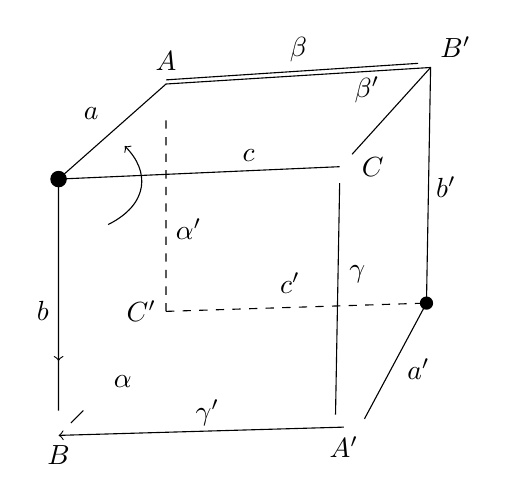
\begin{tikzpicture}[scale=1.05]
\draw (0,0.3)--(0,3.1)--(3.4,3.25);
\draw[->] (0,2.2)--(0,.9);
\draw (0,3.1)--(1.3,4.25)--(4.5,4.45)--(4.45,1.6);
\draw (1.3,4.3)--(4.35,4.5);
\draw (3.55,3.4)--(4.5,4.45) (3.4,3.05)--(3.35,.25) (3.7,.2)--(4.45,1.6);
\draw[<-] (0,0)--(3.45,.1);
\draw[dashed] (1.3,1.5)--(4.45,1.6) (1.3,1.5)--(1.3,3.9);
\draw (.15,.15)--(.3,.3);
\fill (0,3.1) circle(.1);\fill (4.45,1.6) circle(.08);
\draw[->] (.6,2.55)..controls (1.1,2.8) and (1.1,3.2)..(.8,3.5);
\node[above] at (1.3,4.3) {$A$};\node[above right] at (4.5,4.45) {$B'$};
\node[right] at (3.55,3.25) {$C$};\node[left] at (1.3,1.5) {$C'$};
\node[below] at (0,0) {$B$};\node[below] at (3.45,.1) {$A'$};
\node[above left] at (.6,3.7) {$a$};\node[left] at (0,1.5) {$b$};
\node[above] at (2.3,3.2) {$c$};\node[right] at (4.45,3) {$b'$};
\node[right] at (4.1,.8) {$a'$};\node[above] at (2.8,1.6) {$c'$};
\node[right] at (1.3,2.5) {$\alpha'$};\node[right] at (.55,.65) {$\alpha$};
\node[above] at (2.9,4.4) {$\beta$};\node[above left] at (4,3.9) {$\beta'$};
\node[right] at (3.4,1.95) {$\gamma$};\node[above] at (1.8,0) {$\gamma'$};
\end{tikzpicture}}
\[\gamma'-c=a'-\beta'=c'-\beta=\alpha-a\ \big|\ =\delta'\]
\[\left\{\begin{aligned}
\gamma'&=\delta'+c\\
\beta'&=-\delta'+a'\\
\beta&=-\delta'+c'\\
\alpha&=\delta'+a
\end{aligned}\right.\]
\unsure{reste pour expr.} $\uline{\gamma},\uline{\alpha'}$
\[\uline{b-\gamma}=\uline{\alpha-a'}=\uline{\alpha'-b'}=a-\beta'\ \big|\ =\delta''\]
\[\left\{\begin{aligned}
\gamma&=\deleted{\unsure{b}}+\delta''+b\\
\alpha'&=-\delta''+b'
\end{aligned}\right.\]
\[\begin{aligned}
\alpha&=-\delta^{\unsure{''|4}}+a'\\
\beta'&=\unsure{\vert|1}+\delta^{\unsure{''|4}}+a
\end{aligned}\]
\[\boxed{-\delta''+a'=\delta'+a}\]
\figure{\begin{tikzpicture}\node[draw,ellipse] {$\delta'+\delta^{\unsure{''|4}}=a'-a$};\end{tikzpicture}}
\[\boxed{+\delta^{\unsure{''|4}}+a=-\delta'+a'}\]
\margin{212}
\scanpage{214}
\mspage{451}
résiste pas à la tentation de la reproduire ici\inserted{(traduite)} in extenso\inserted{.}\deleted{\unsure{--}} \deleted{i}\inserted{I}l m'a fallu un moment, d'ailleurs, pour saisir que c'\deleted{\unsure{e}}était bel et bien une réponse à ma belle lettre \deleted{\unsure{d'il y avait}} du mois dernier\deleted{\unsure{;}}\inserted{. Voici donc la réponse.}

\begin{flushright}Heidelberg 15.3.1985\end{flushright}
\deleted{``}Cher Professeur Grothendieck,

Il me faut encore vous remercier pour votre lettre du 9 février. La lettre de Mme Dr. Byrne du 15 février aura sans doute répondu à vos questions.

\unsure{Recevez} etc
\begin{flushright}K.F. Springer\deleted{''}\end{flushright}

Là au moins je suis fixé ! Les gens ``bien informés'' (dont il a été déjà question) ont dû lui expliquer que c'était pas la peine qu'il se fatigue pour le Monsieur un peu excité qui lui écrivait là -- qu'il\deleted{\unsure{b}} ne faisait décidément pas partie du beau monde. Et c'est vrai, en plus ...

En attendant de recevoir cette réponse édifiante de la direction de l'entreprise de Pompes Funèbres Springer Verlag GmbH (c'était gentil encore de m'honorer d'une réponse \deleted{personelle}\inserted{signée} du directeur en personne), j'ai eu le temps de me sonder sur mes propres intentions. Le rôle joué par l'estimable entreprise me paraît vraiment très gros, et j'ai songé à l'éventualité d'un procès à grand spectacle, où je demanderais des dommages-intérêts astronomiques, à titre de ``monsieur bien''\inserted{ }outragé, \deleted{et} victime d'inqualifiables passes\deleted{\unsure{x}}-droits. Mais je me suis dit aussi \deleted{\unsure{que de tels pro}} qu'un procès comme ça, ça doit bouffer une énergie\inserted{ }dingue. A supposer même que j'aie gain de cause et que je touche des dommages-intérêts vertigineux (soyons optimistes!)\inserted{,} au bout de X années\deleted{,}\inserted{\unsure{certes,|civils,}} -- à quoi serais-je avancé ? Je ne suis pas dans le besoin et n'ai nul besoin de plus que ce que j'ai -- et une escroquerie n'est pas plus ni moins une escroquerie, parce qu'un certain procès a été gagné, ou perdu. Je ne vais pas améliorer le monde, ni moi-même, ni les manières de Monsieur K.F. Springer et de certains employés de l'entreprise qu'il dirige, et en tous cas pas leur\deleted{s} façon de concevoir leur métier\inserted{,} en mobilisant des avocats et en \deleted{le}\inserted{leur} faisant mobiliser les leurs\inserted{(*)}. \deleted{\unsure{Par contre, dans les années qui m}} Et je n'améliorerai pas non plus un certain esprit dans un certain beau monde que j'ai quitté, \deleted{un}\inserted{l'} esprit qui rend possible le genre d'opération dont le Dr. Springer et son estimable \deleted{entre} maison se sont\inserted{faits (depuis \unsure{treize|douze} ans) \deleted{\unsure{déjà}}} les serviteurs. Il me reste (je l'espère bien) quelques
\margin{213}
\scanpage{215}
\[b-\alpha'=\gamma'-c'=\gamma-b'=c-\beta=-\delta\]
\[\begin{aligned}
\alpha'&=\delta+b\\
\gamma'&=-\delta+c'\\
\gamma&=-\delta+b'\\
\beta&=\delta+c
\end{aligned}\]
\[\boxed{\deleted{\delta+b=-\delta''+b'}}\]
\[\boxed{-\delta+c'=\unsure{\delta'}+c}\]
\[\boxed{\deleted{-\delta+b'=\delta''+b}}\]
\[\boxed{\delta+c=-\delta'+c'}\]
\figure{\begin{tikzpicture}\node[draw,ellipse] {$\begin{aligned}
\delta+\delta''&=b'-b\\
\delta+\delta'&=c'-c\deleted{\unsure{\varepsilon}}
\end{aligned}$};\end{tikzpicture}}
\[\begin{aligned}
\delta'+\delta''&=a'-a\\
\delta''+\delta&=b'-b\\
\delta+\delta'&=c'-c
\end{aligned}\]
\figure{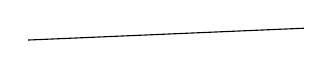
\begin{tikzpicture}\draw (0,0)--(3.5,.15);\end{tikzpicture}}
\[\begin{aligned}
\delta+\delta'+\delta^{\unsure{''|4}}
 &=\frac12\bigl(a'+b'+c'-(a+b+c)\bigr)\\
 &=\frac12\bigl(\underbrace{(a'-a)}_{\varepsilon_1}
 +\underbrace{(b'-b)}_{\varepsilon_2}+\underbrace{(c'-c)}_{\unsure{\varepsilon_2|\varepsilon_3}}\bigr)
\end{aligned}\]
\[\boxed{\left\{\begin{aligned}
\delta&=\frac12(-\varepsilon_1+\varepsilon_2+\varepsilon_3)\\
\delta'&=\frac12(\varepsilon_1-\varepsilon_2+\varepsilon_3)\\
\delta''&=\frac12(\varepsilon_1+\varepsilon_2-\varepsilon_3)
\end{aligned}\right.}\]
\margin{214}
\scanpage{216}
\mspage{450}
(Ce n'est pas\inserted{certes,} la première fois\inserted{(ni la dernière que je suis ``\unsure{soufflé}'' \unsure{)}} dans cette brillante opération ``au service de la science''\inserted{...)}\deleted{\unsure{rôle}\illegible{5}}. J'apprends par sa lettre (datée du 15 février 85) que conformément \deleted{aux} ``à la façon habituelle d'agir quand un ouvrage contient des contributions de plusieurs auteurs'' (sic), il n'y avait pas lieu de s'adresser plus spécialement à moi, qui n'étais que \uline{directeur} du Séminaire ... \deleted{(}Les cinq ``auteurs'' de SGA 5 sont Bucur, Houzel, Illusie, Jouanolou, Serre, à l'exclusion de ma modeste personne, qui \deleted{ne} ne figure que comme ``directeur'' -- sans doute purement honorifique, en \deleted{ais}\inserted{avais}-je trop dit (*) -- pour ce brillant séminaire.

Dès avant de recevoir cette lettre instructive et trouvant le temps long (n'ayant rien reçu pendant un mois), j'ai pris ma plus belle plume (en allemand) pour écrire au Dr. K.F Springer en personne, \inserted{lequel} fai\deleted{san}t partie des directeurs responsables de la maison Springer. Ça a été une belle \deleted{\unsure{lett}} lettre de deux pages machine, lui expliquant que j'étais bien peiné d'une longue série de désagréments dans ma relation à la maison Springer, et au delà de celles-ci, d'un certain nombre d'irrégularités grossières à mon égard, dont je me contentais pour le moment de lui soumettre deux, qui me paraissaient particulièrement flagrant\deleted{s}\inserted{es}: la publication de deux volumes des Lecture Notes (n\textsuperscript{o}s 288,589) parus sous mon nom et sans \deleted{aucun} juger nécessaire de me consulter. Que dans ces deux \deleted{cas}\inserted{textes}, les idées, méthodes et résultats que j'avais développés dans les séminaires oraux, étaient raccourcis ou mutilés parfois au point d'être méconnaissables. Que la coïncidence de ce dernier fait, \inserted{avec} \deleted{d}\inserted{l}es circonstances inhabituelles qui ont entouré la publication de ces deux volumes, ne pouvait être pour moi l'effet d'un pur hasard. Et que je m'attendais à des excuses publiques\deleted{, de la part} et sans réserve de la part de la maison\inserted{ }Springer, sous une forme qui serait à fixer d'un commun accord, une fois \deleted{que la question}\inserted{qu'un accord} de principe \deleted{était}\inserted{\unsure{serait}} acquis. Que j'espérais qu'il aurait à coeur comme moi de mettre fin à une situation déplaisante et inadmissible et de trouver une solution\unsure{n}qui soit à la hauteur des circonstances (``eine dem Fall geziemende Lösung zu finden'', ce qui \deleted{est} est même plus distingué encore), ``ho\deleted{\unsure{a}}chachtungsvoll'' (comme il se doit) signé de ma plus belle main.

Pour jouer cartes sur table, il me semble que j'ai joué cartes sur table ! Là il ne pourra pas dire, Monsieur K.F. Springer, qu'il \unsure{n'a} pas été informé personnellement de la situation, et de première main encore\deleted{\unsure{k}}\inserted{,} par nul autre que le principal intéressé lui-même!

Le hasard fait bien les choses: j'ai \deleted{\unsure{réçu|reçu}} fini par recevoir une réponse (un bon mois après\inserted{encore}) pas\inserted{\unsure{,}}plus tard que hier. C'est si court que je ne
\margin{215}
\scanpage{217}
\diagram{\begin{tikzcd}[ampersand replacement=\&, row sep=large]
\alpha=\sigma_{BC'}=\frac12\bigl((\uline{a'+a})\unsure{-|+}(b'-b)+(c'-c)\bigr)\ \bullet\arrow[dd,bend left=55]\\
\beta=\sigma_{AB'}=\frac12\bigl(-(a'\unsure{-|+}a)+(b'-b)+(\uline{c'+c})\bigr)\arrow[u,bend right=30]\\
\gamma=\sigma_{CA'}=\frac12\bigl((a'-a)+(\uline{b'+b})-(c'-c)\bigr)\arrow[u,bend right=30]
\end{tikzcd}}
\diagram{\begin{tikzcd}[ampersand replacement=\&, row sep=large]
\alpha'=\sigma_{AC'}=\frac12\bigl(-(a'-a)+(\uline{b+b^{\unsure{3|'}}})+(c'-c)\bigr)\arrow[dd,bend left=55]\\
\beta'=\sigma_{CB'}=\frac12\bigl((a'+a)+(b'-b)-(\unsure{c}c'-c)\bigr)\ \bullet\arrow[u,bend right=30]\\
\gamma'=\sigma_{BA'}=\frac12\bigl((a'-a)\unsure{-|+}(b'-b)+(c'+c)\bigr)\arrow[u,bend right=30]
\end{tikzcd}}
\margin{\[
\begin{gathered}-c'+c+2c'\\-b'+b\\-a'+a\\c'-c\end{gathered}\]}
\unsure{Sommes} des $\sigma_a$ sur les arêtes d'une face
\[\begin{aligned}
\varphi_a&=\deleted{\unsure{b+c+}}(a'-a)+2(b+c)\\
\varphi_b&=(b'-b)+2(a+c)\\
\varphi_c&=(c'-c)+2(a+b)
\end{aligned}\]
\figure{\begin{tikzpicture}\draw[->] (0,0)--(0,-3.5);\end{tikzpicture}}
\[a-a'+(b'+c')\]
\diagram{\begin{tikzcd}[ampersand replacement=\&, column sep=.1em,row sep=large]
\varphi_{a'}=(b'+c')\unsure{-|=}(a'-a)+b'+c'=\&2\&(b'+c')-(a'-a)\\
\varphi_{b'}=a'+c'+a'-(b'-b)+c'=\&2\&(c'+a')-(b'-b)\\
\varphi_{c'}=(\unsure{a'}+b')+a'+b'-(c'-c)=\&2\&(a'\unsure{+|-}b')-(c'-c)\\
\&\makebox[0pt]{\deleted{\unsure{le facteur 2 est partout !|les signes sont partout !}}}
\arrow[uuu,bend left=45]\arrow[uu,bend left=30]\arrow[u,bend left=15]\&
\end{tikzcd}}
\margin{216}
\scanpage{218}
\mspage{L 21}
quand ce n'était celui du dédain (``délicatement dosé''), de la dérision ou du mépris, que ce soit vis-à-vis de moi (parfois) ou (surtout) vis-à-vis de ceux qui avaient osé s'inspirer de moi (sans se douter, certes, de ce qui les attendait) et qui étaient ``classés'' comme ayant partie liée à moi, par quelque décret tacite et implacable. Et à nouveau je vois apparaître ici le lien ``évident'' et profond, entre le r\enspace e\enspace s\enspace p\enspace e\enspace c\enspace t (ou l'absence de respect) pour la personne d'autrui, celui pour l'acte de création et pour certains de ses fruits \deleted{parmi} les plus délicats et les plus essentiels, et enfin le respect pour les règles les plus évidentes de l'éthique scientifique, celles qui s'enracinent dans un respect élémentaire de soi et d'autrui et que je serais tenté d'appeler les ``r\enspace è\enspace g\enspace l\enspace e\enspace s\quad d\enspace e\quad d\enspace é\enspace\deleted{\unsure{c|e}}\enspace c\enspace e\enspace n\enspace c\enspace e'' dans l'exercice de notre art. \inserted{Ce sont là autant d'aspects, sûrement, d'un élémentaire et essentiel ``\uuline{respect} \uline{de soi}''.} Si j'essaie, en une seule formule lapidaire\inserted{,} de faire le bilan de ce que m'a enseigné Récoltes et Semailles au sujet d'un certain monde qui fut le mien, un monde auquel je m'étais identifié pendant plus de vingt ans de ma vie, je dirais: c'est un monde qui a p\enspace e\enspace r\enspace d\enspace u\quad l\enspace e\quad r\enspace e\enspace s\enspace p\enspace e\enspace c\enspace t (*).

C'était là une chose déjà fortement sentie, sinon formulée, dès les années qui avaient précédé. Elle n'a fait que se confirmer et se préciser\inserted{,} de façon \deleted{souvent} imprévue toujours et parfois stupéfiante, tout au cours de Récoltes et Semailles. Elle est clairement apparente dès le moment déjà où une réflexion de nature ``philosophique'' et générale devient soudain un témoignage personnel, dans la section ``L'étranger bienvenu'' (n° $9\deleted{\unsure{5}}$, p. 18) ouvrant le chapitre déjà cité ``Naissance de la crainte''\deleted{)}.

Cette perception n'apparaît pourtant pas sur le ton de la récrimination acerbe ou amère, mais (par la logique interne de l'écriture et par l'attitude différente que celle-ci suscite) sur celui d'une i\enspace n\enspace t\enspace e\enspace r\enspace r\enspace o\enspace g\enspace a\enspace t\enspace i\enspace o\enspace n : quelle a été ma propre part dans cette dégradation, dans cette perte du respect que je constate aujourd'hui ? C'est là l'interrogation principale qui traverse et porte cette première partie de\margin{\unsure{(!)}} Récoltes et Semailles, jusqu'au moment où elle se résoud finalement en une constatation claire et sans équivoque (**). Auparavant, cette dégradation m'était apparue comme ``tombée du ciel'' soudain, de façon inexplicable et d'autant plus outrageuse, intolérable. Au cours de la réflexion, je découvre qu\deleted{e}\inserted{'} \deleted{cette}\inserted{elle} \deleted{dégradation} s'était \deleted{déjà} poursuivie insidieusement, sans que personne sûrement ne la décèle autour de lui ni en lui-même, tout au \deleted{cours}\inserted{long} des années cinquante et soixante, y\quad c\enspace o\enspace m\enspace p\enspace r\enspace i\enspace s\quad d\enspace a\enspace n\enspace s\quad m\enspace a\quad p\enspace r\enspace o\enspace p\enspace r\enspace e\quad p\enspace e\enspace r\enspace s\enspace o\enspace n\enspace n\enspace e.

\deleted{\unsure{Cette constat}} La constatation de cet humble fait,\inserted{bien} évident sûrement
\margin{217}
\scanpage{219}
\[\begin{aligned}
&\begin{array}{c}
\begin{array}{rrrrrr}a&b&c&a'&b'&c'\end{array}\\[.3em]
\det\left(\begin{array}{|rrr|rrr|}\hline
\unsure{-1}&2&2&1&0&0\\
2&-1&2&0&1&0\\
2&2&-1&0&0&1\\\hline
1&0&0&-1&2&2\\
0&1&0&2&-1&2\\
0&0&1&2&2&-1\\\hline
\end{array}\right)
\end{array}
=\det\begin{pmatrix}27&1\\1&27\end{pmatrix}\\
&=27^2-1\in\mathbb Q^*\\
&=(3^3)^2-1=3^6-1\\
&=728\\
&=8.91\\
&\boxed{=2^3.7.13}
\end{aligned}\]
\uline{premier à $3$}
\[-1+8+8-(-4-4-4)=16+12-1=27\]
\unsure{OK}
\[\deleted{\unsure{27}}\]
\diagram{\(\begin{array}{rrr}
&2&7\\
&2&7\\\hline
1&8&9\\
5&4&\\\hline
7&2&9
\end{array}\)}
\margin{218}
\scanpage{220}
\margin{\unsure{1}}
\mspage{L 20}
\deleted{par des épithètes} comme ``vaseux'', ``mou'', ``inconsistant'' -- ou au bout opposé\inserted{comme} ``trivialités'', ``enfantillage'', ``\unsure{bonbinage|bombinage}'' ...), mais où sera extirpé également ce travail même et ses fruits: celui où sont conçues, s'élaborent et naissent les notions et les visions nouvelles. Ce sera l'époque aussi où l'exercice de notre art sera réduit à d'arides et vaines voltiges de ``poids et haltères'' cérébraux, aux surenchères des prouesses pour ``craquer'' les problèmes au concours (``de difficulté proverbiale'') -- l'époque d'une hypertrophie ``supermacho'' fiévreuse et stérile, prenant la suite de plus de trois siècles de renouvellement créateur.

\inserted{7.} Mais à nouveau je digresse, en anticipant sur ce que la réflexion m'a enseigné. \deleted{Je}\inserted{J'étais} part\deleted{ais}\inserted{i} d'un double propos\inserted{,} clairement présent en moi dès avant même les débuts de celle-ci: le propos d'une ``déclaration d'intentions'', et (intimement lié à celui-ci, comme il vient d'apparaître) celui de m'exprimer au sujet de la nature du travail créateur. Il y avait pourtant un troisième propos encore, moins clairement présent sûrement au niveau conscient, mais répondant à un besoin \unsure{pbus|plus} profond et plus essentiel. Il était suscité par ces ``interpellations'' parfois déconcertantes, me \unsure{pervenant|parvenant} de mon passé de mathématicien par la voix de ceux qui avaient été mes élèves ou mes amis\unsure{(} (ou \deleted{les deux}\inserted{du moins}, de \deleted{certains}\inserted{bon nombre} d'entre eux). Au niveau épidermique, ce besoin se traduisait par une envie de ``vider mon sac'', de dire quelques ``vérités déplaisantes''. Mais plus profondément, sûrement, il y avait le besoin de \deleted{faire} f\enspace a\enspace i\enspace r\enspace e\quad c\enspace o\enspace n\enspace n\enspace a\enspace i\enspace s\enspace s\enspace a\enspace n\enspace c\enspace e enfin avec un certain passé, que j'avais choisi jusque là d'éluder. C'est de ce besoin-là, avant tout, qu'est \deleted{né}\inserted{issu} Récoltes et Semailles. Cette longue réflexion a été ma ``réponse'', au jour le jour, à cette pulsion de connaissance en moi, et à l'interpellation sans cesse renouvelée qui me venait du monde extérieur, du ``monde mathématique'' que j'avais quitté sans esprit de retour. Mais à part les toutes premières pages de ``Fatuité et Renouvellement''\deleted{,}\inserted{(}celles qui en forment les deux premiers chapitres ``Travail et découverte'' et ``Le rêve et le Rêveur''\inserted{)}, et dès le chapitre qui enchaîne ``Naissance de la crainte'' (p. 18), avec un ``témoignage'' qui n'était nullement prévu au programme, c'est ce besoin de faire connaissance de mon passé et de l'assumer pleinement, qui (je crois) a été la force principale en oeuvre dans l'écriture de Récoltes et Semailles.
\deleted{Récoltes et Semailles}

L'interpellation qui m'était venue du monde des mathématiciens, et qui revenait sur moi avec une force nouvelle tout au cours \deleted{de l'écriture} de Récoltes et Semailles (et surtout,\inserted{au cours} de l' ``enquête'' poursuivie dans les parties II et IV) avait pris d'emblée le masque de la suffisance,
\margin{219}
\scanpage{221}
\[
\begin{aligned}
 A&=a+a'=\lambda\\
 B&=b+b'=\mu\\
 C&=c+c'=\nu
\end{aligned}
\qquad
\boxed{\lambda,\mu,\nu}\quad\text{correspondent aux trois directions d'arêtes}
\]
\[
\deleted{\unsure{\beta}}\qquad
\begin{aligned}
 A'&=a'\unsure{+|-}a\\
 B'&=b'-b\\
 C'&=c'\unsure{+|-}c
\end{aligned}
\qquad\uline{\lambda\ \mu\ \nu}
\]
\figure{\begin{tikzpicture}[x=1cm,y=1cm]
\draw (-1.5,.8)--(-1.4,-.25);
\fill (-1.54,.22) circle(.025);
\draw (.2,2)--(.2,1.05);
\draw (.23,1.8)--(.37,1.5)--(.46,1.5)--(.7,.35);
\draw (.7,-.05)--(.82,-1.2);
\fill (.68,-.55) circle(.025);
\draw (1.65,1.05)--(1.72,-.3);
\fill (1.7,.48) circle(.025);
\end{tikzpicture}}
\[
\begin{aligned}
 a\unsure{+|-}a'&=\lambda\\
 b\unsure{+|-}b'&=\mu\\
 c\unsure{+|-}c'&=\nu
\end{aligned}
\qquad
\varphi_a+\varphi_{a'}=2(b+b'\unsure{-|+}c+c')=2(\mu+\nu)
\]
\margin{220}
\scanpage{222}
\margin{221}
\mspage{L 19}
Récoltes et Semailles j'ai pu me rendre compte, et de façon saisissante en ces tout derniers mois surtout (avec l'écriture des Quatre Opérations), qu'il y a eu depuis mon départ de la scène mathématique une stupéfiante d\enspace é\enspace g\enspace r\enspace a\enspace d\enspace a\enspace t\enspace i\enspace o\enspace n dans l'esprit qui aujourd'hui fait loi dans les milieux \unsure{qye|que} j'avais connus, et (me semble-t-il, dans une large mesure au moins) dans le monde mathématique en général (*). Il est possible même,\deleted{\unsure{que}} tant par ma personnalité mathématique très particulière que par les conditions qui ont entouré mon départ, que celui-ci ait agi comme un catalyseur dans une évolution qui était déjà en train de se faire (**) -- une évolution dont je n'ai\inserted{alors} rien su percevoir (pas plus qu'aucun autre de mes collègues et amis, à la seule exception peut-être de Claude Chevalley). L'aspect de cette dégradation auquel je pense surtout ici (qui\inserted{en} est\inserted{\unsure{juste|partie}} \uline{un} aspect parmi de nombreux autres (***)) est le m\enspace é\enspace p\enspace r\enspace i\enspace s\quad t\enspace a\enspace c\enspace i\enspace t\enspace e, quand ce n'est la dérision sans équivoque, à l'encontre de ce qui (en mathématique, en l'occurrence) ne s'apparente pas au pur travail du marteau sur l'enclume ou sur le burin -- le mépris des processus créateurs les plus délicats (et \deleted{\unsure{parf}} souvent de moindre apparence\inserted{)}; de tout ce qui est \deleted{\unsure{inspiration}} i\enspace n\enspace s\enspace p\enspace i\enspace r\enspace a\enspace t\enspace i\enspace o\enspace n, r\enspace ê\enspace v\enspace e, v\enspace i\enspace s\enspace i\enspace o\enspace n (si puissantes et si fertiles soient-elles), et même (à la limite) de toute i\enspace d\enspace é\enspace e, si clairement conçue et formulée soit-elle : de tout ce qui n'est écrit et p\enspace u\enspace b\enspace l\enspace i\enspace é noir sur blanc, sous forme d'énoncés purs et durs, répertoriables et répertoriés, mûrs pour les ``banques de données'' \deleted{\unsure{s'}}engouffrés dans les inépuisables mémoires de nos mégaordinateurs.

Il y a eu (pour reprendre une expression de C.L. Siegel (\unsure{****}) un extraordinaire \deleted{``\unsure{aplatissement}''}\inserted{``a\enspace p\enspace l\enspace a\enspace t\enspace i\enspace s\enspace s\enspace e\enspace m\enspace e\enspace n\enspace t''}, un ``r\enspace é\enspace t\enspace r\enspace é\enspace c\enspace i\enspace s\enspace s\enspace e\enspace m\enspace e\enspace n\enspace t'' de la pensée mathématique,\deleted{\unsure{f}} dépouillée d'une dimension essentielle, de tout son ``versant d'ombre'', du versant ``féminin''. Il est vrai que par une tradition ancestrale, ce versant-là du travail de découverte restait dans une large mesure\inserted{ }occulté, personne (autant dire) n'en p\enspace a\enspace r\enspace l\enspace a\enspace i\enspace t jamais -- mais le contact\inserted{vivant} avec les sources profondes du rêve, qui alimentent les grandes visions et les grands desseins, n'avait jamais encore (à ma connaissance) été perdu. Il semblerait que\inserted{dès à} présent nous soyons déjà entrés dans une é\enspace p\enspace o\enspace q\enspace u\enspace e\quad d\enspace e\quad d\enspace e\enspace s\enspace s\enspace è\enspace c\enspace h\enspace e\deleted{\unsure{men}}\enspace m\enspace e\enspace n\enspace t, où cette source est, non point tarie certes, mais où l'accès à elle est condamné\deleted{\unsure{s}}, par le verdict sans appel du mépris général et par les représailles de la dérision.

\inserted{\figure{\begin{tikzpicture}[scale=.3]\draw[blue] (0,0)--(1.2,0)--(1.2,1)--(3.3,1);\draw[blue] (1.05,0)--(1.05,1);\end{tikzpicture}}}
Nous voilà approcher du moment, semble-t-il, où sera éradiqué en chacun non seulement le s\enspace o\enspace u\enspace v\enspace e\enspace n\enspace i\enspace r de tout travail proche de la source, du travail ``au féminin'' (ridiculisé
